%!TEX root = /Users/stevenmartell/Documents/iSCAM-project/fba/Halibut/WRITEUP/Halibut.tex
\section{Results} % (fold)
\label{sec:results}

\subsection{Impacts of MSL on exploitable biomass} % (fold)
\label{sub:impacts_of_msl_on_exploitable_biomass}

Decreasing the minimum size limit from 32 inches to 26 inches results in a 2 million pound increase in the average simulated exploitable biomass between the years 2020 and 2025 (Figure \ref{fig:FIGURES_SIZELIMIT_fig_32_DI_EBio}).  Note that the exploitable biomass calculation is based on the product of the numbers-at-age, the weight-at-age, and the age-specific capture probabilities (commercial fishery selectivity).  Under density-independent growth, exploitable biomass is highest for the good recruitment scenarios; whereas, under density-dependent growth larger exploitable biomass is expected due to growth compensation at low densities (note red \& blue lines in Figure \ref{fig:FIGURES_SIZELIMIT_fig_32_DI_EBio}).  



\begin{figure}[htbp]
	\centering
		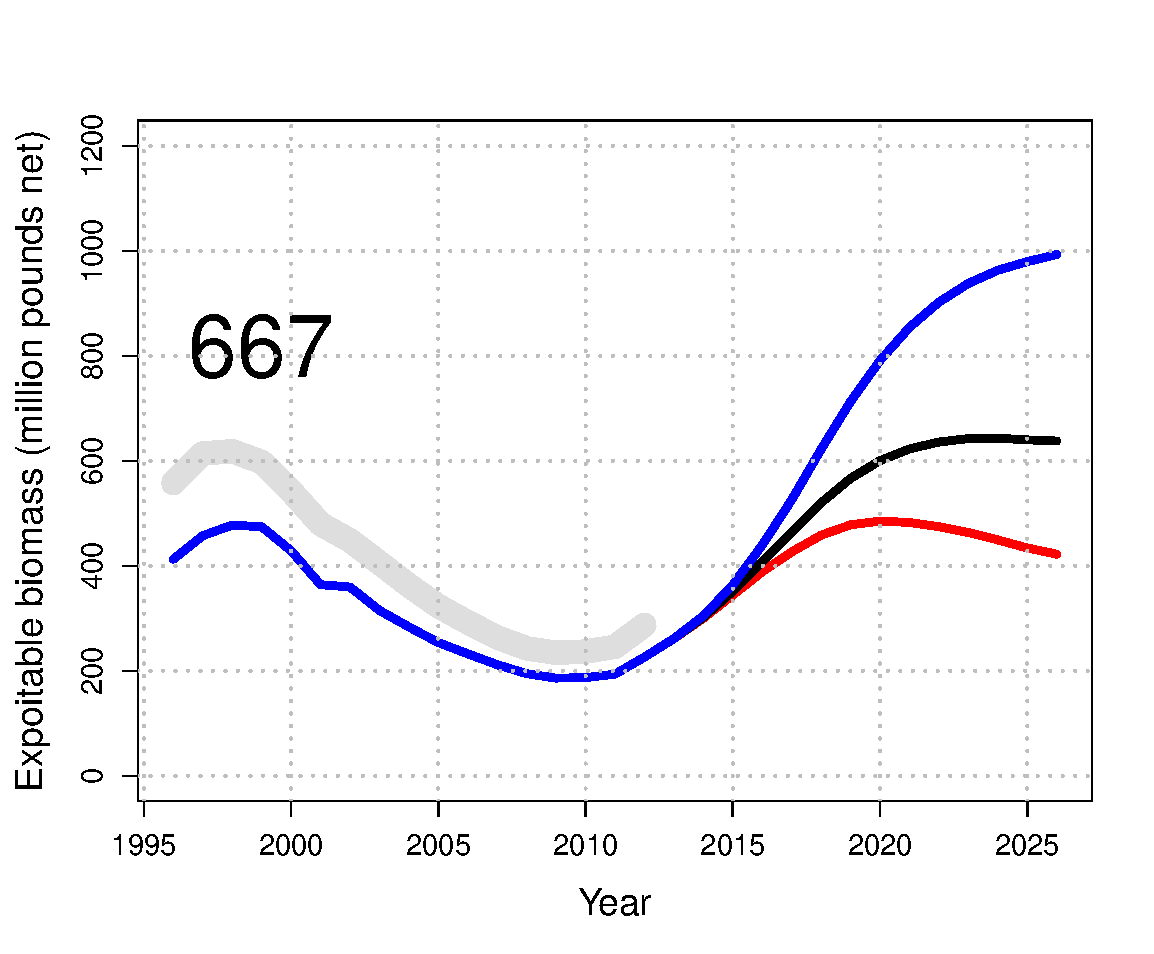
\includegraphics[height=1.5in]{../FIGURES/SIZELIMIT/fig_32_DI_EBio.pdf}
		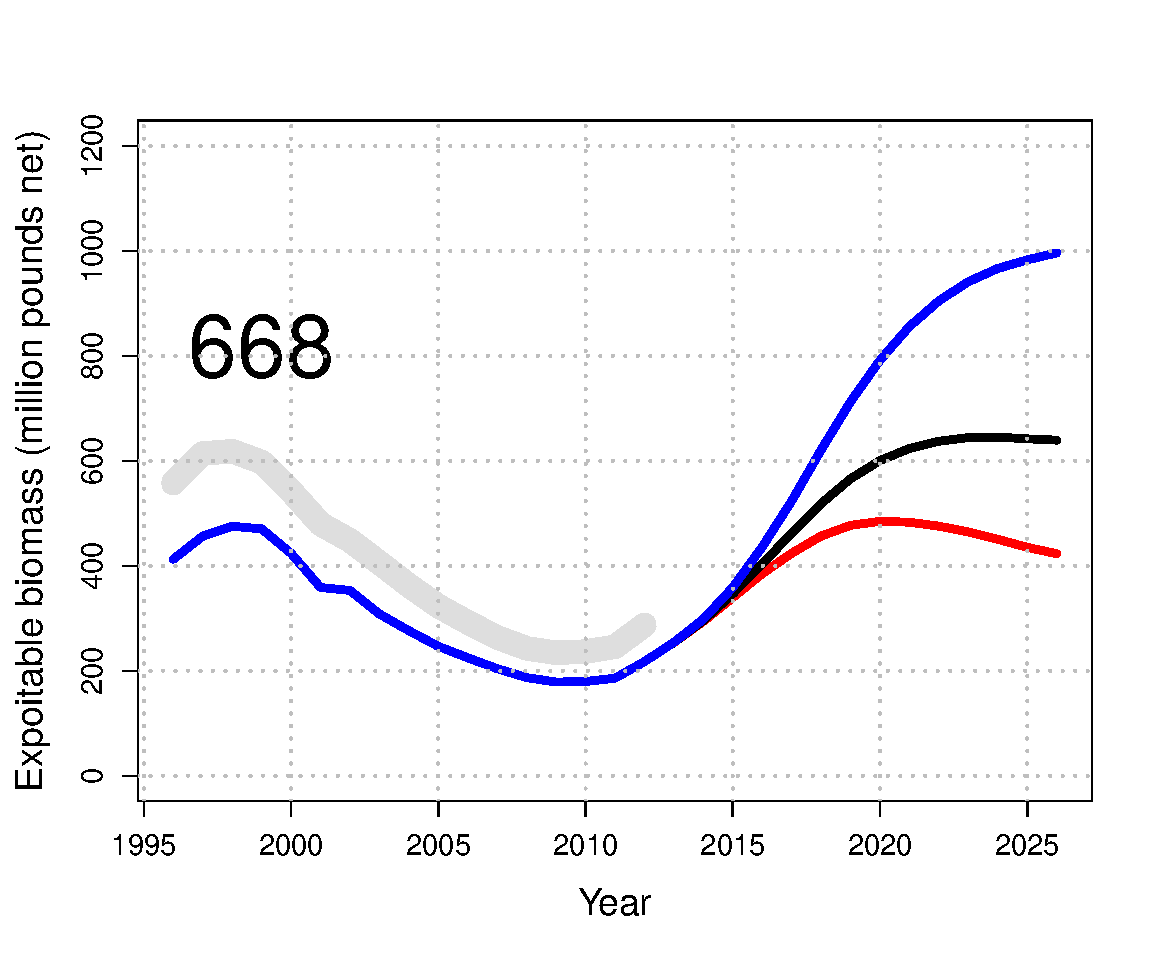
\includegraphics[height=1.5in]{../FIGURES/SIZELIMIT/fig_29_DI_EBio.pdf}
		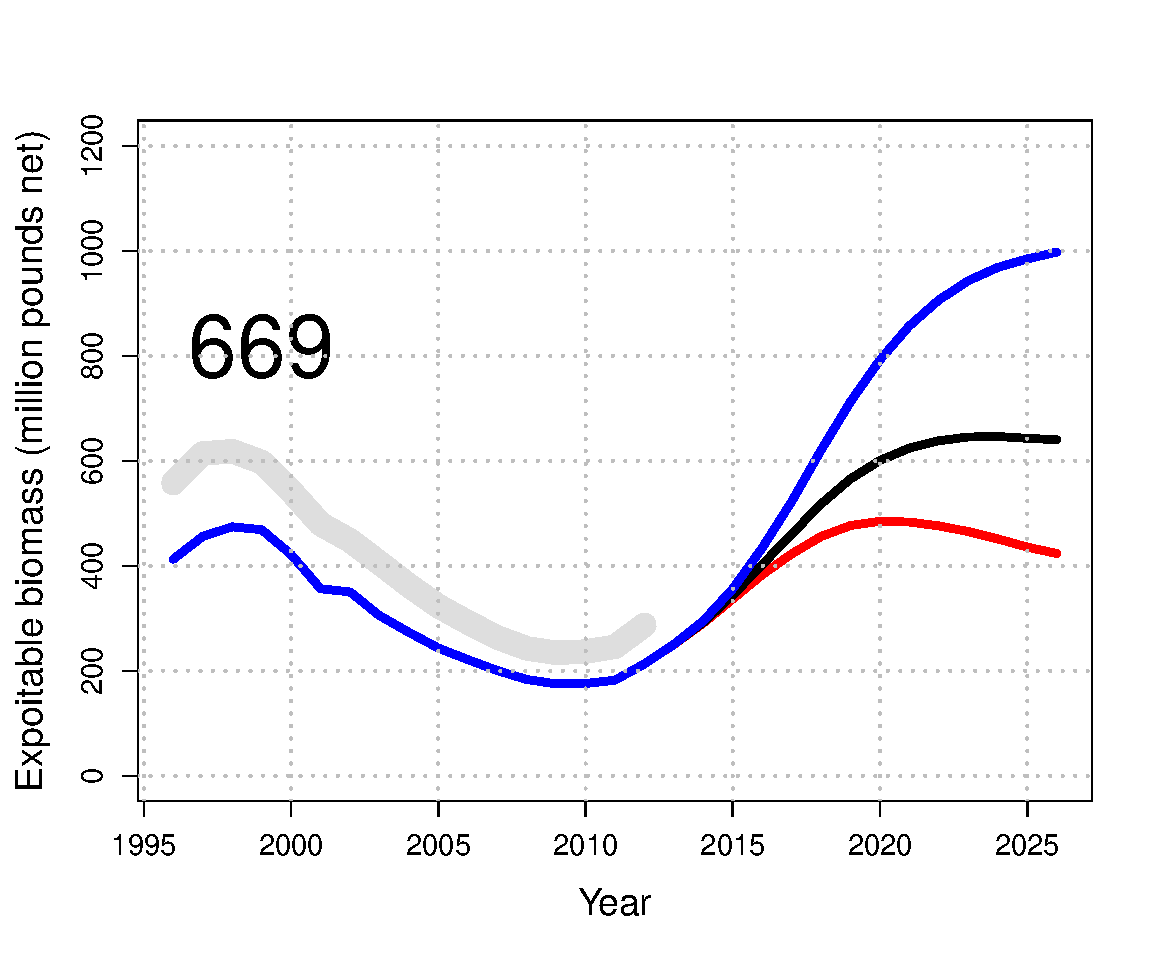
\includegraphics[height=1.5in]{../FIGURES/SIZELIMIT/fig_26_DI_EBio.pdf}
		
		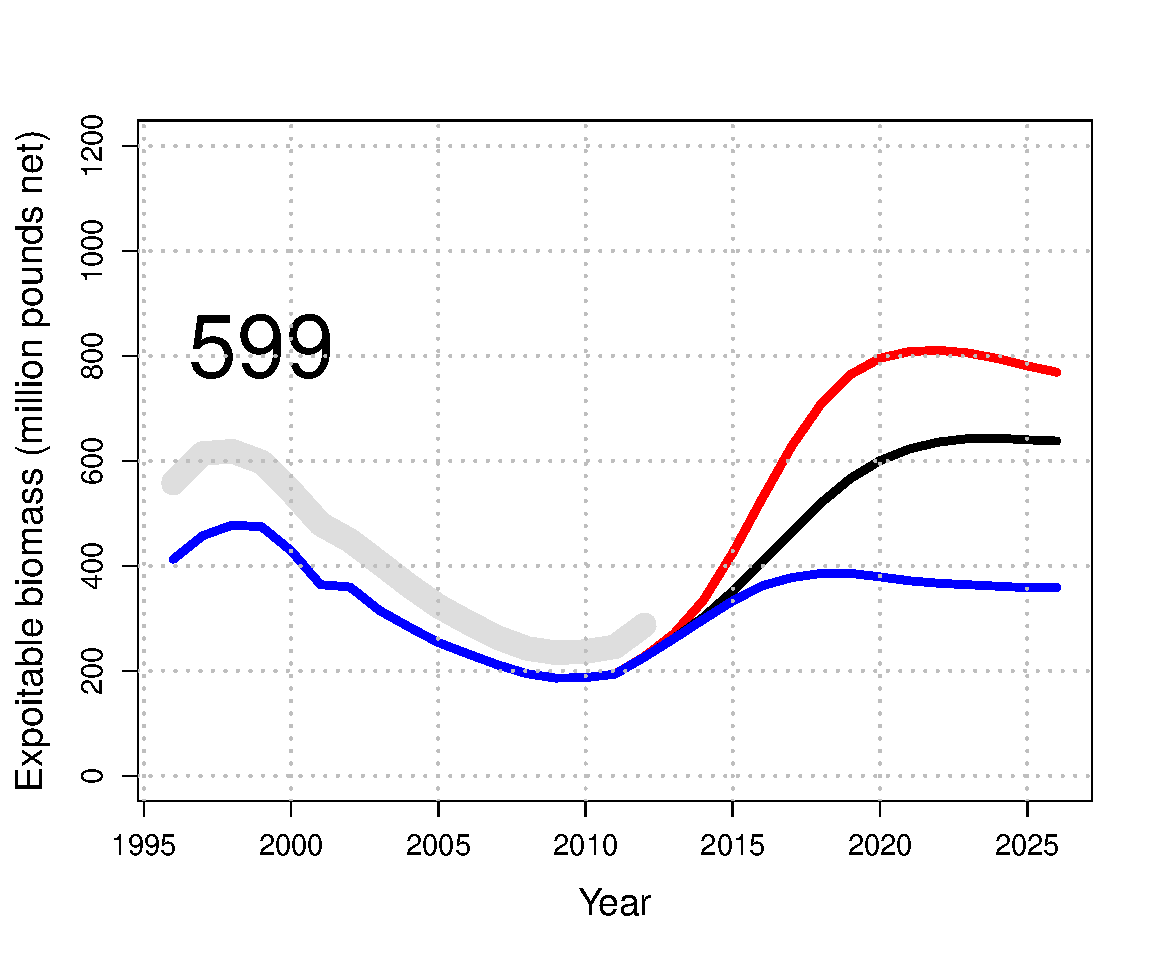
\includegraphics[height=1.5in]{../FIGURES/SIZELIMIT/fig_32_DD_EBio.pdf}
		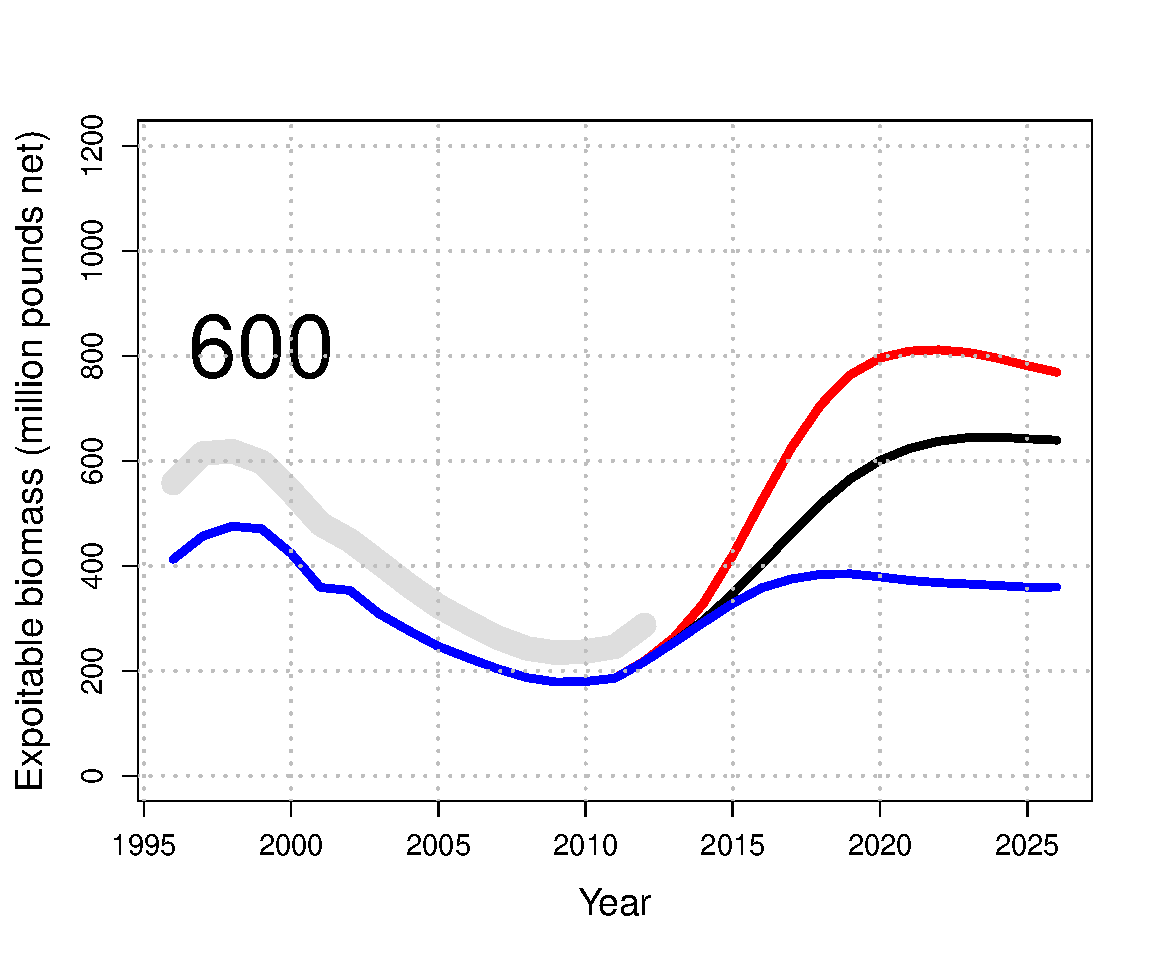
\includegraphics[height=1.5in]{../FIGURES/SIZELIMIT/fig_29_DD_EBio.pdf}
		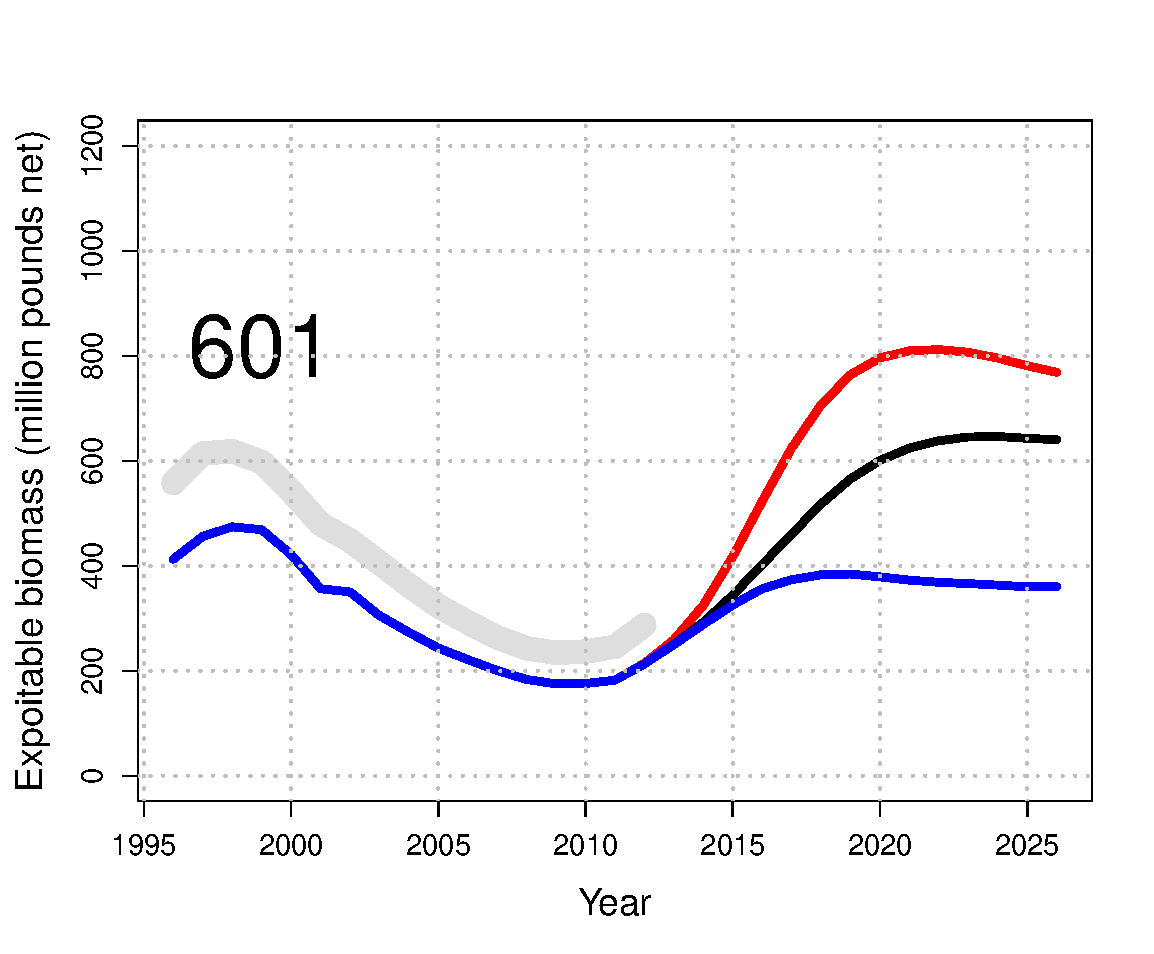
\includegraphics[height=1.5in]{../FIGURES/SIZELIMIT/fig_26_DD_EBio.pdf}
	\caption{Effects of MSL on exploitable biomass under the assumptions of density-independent growth (top row) and density-dependent growth (bottom row) for 32 inch (left), 29 inch (middle), and 26 inch (right) size limits.  Poor, average, and good recruitment are denoted by red, black and blue lines, respectively.  Value on each panel corresponds to 2020-2025 average over 3 recruitment hypotheses.}
	\label{fig:FIGURES_SIZELIMIT_fig_32_DI_EBio}
\end{figure}

% subsection impacts_of_msl_on_exploitable_biomass (end)
\subsection{Impacts of MSL on commercial yield} % (fold)
\label{sub:impacts_of_msl_on_commercial_yield}
A modest increase of 300,000 to 500,000 pounds in the  average coastwide commercial yields (between the years 2020--2025) is projected with a decrease in the minimum size limit from 32 inches to 26 inches (Figure \ref{fig:FIGURES_SIZELIMIT_fig_32_DI_YBio}).  This increase owes to the overall reduction in total mortality rates associated with commercial wastage.  Note also that these results also assume that bycatch levels and removals by the recreational fishery and personal use, including subsistence harvest, remains at the 2011 levels.


\begin{figure}[htbp]
	\centering
		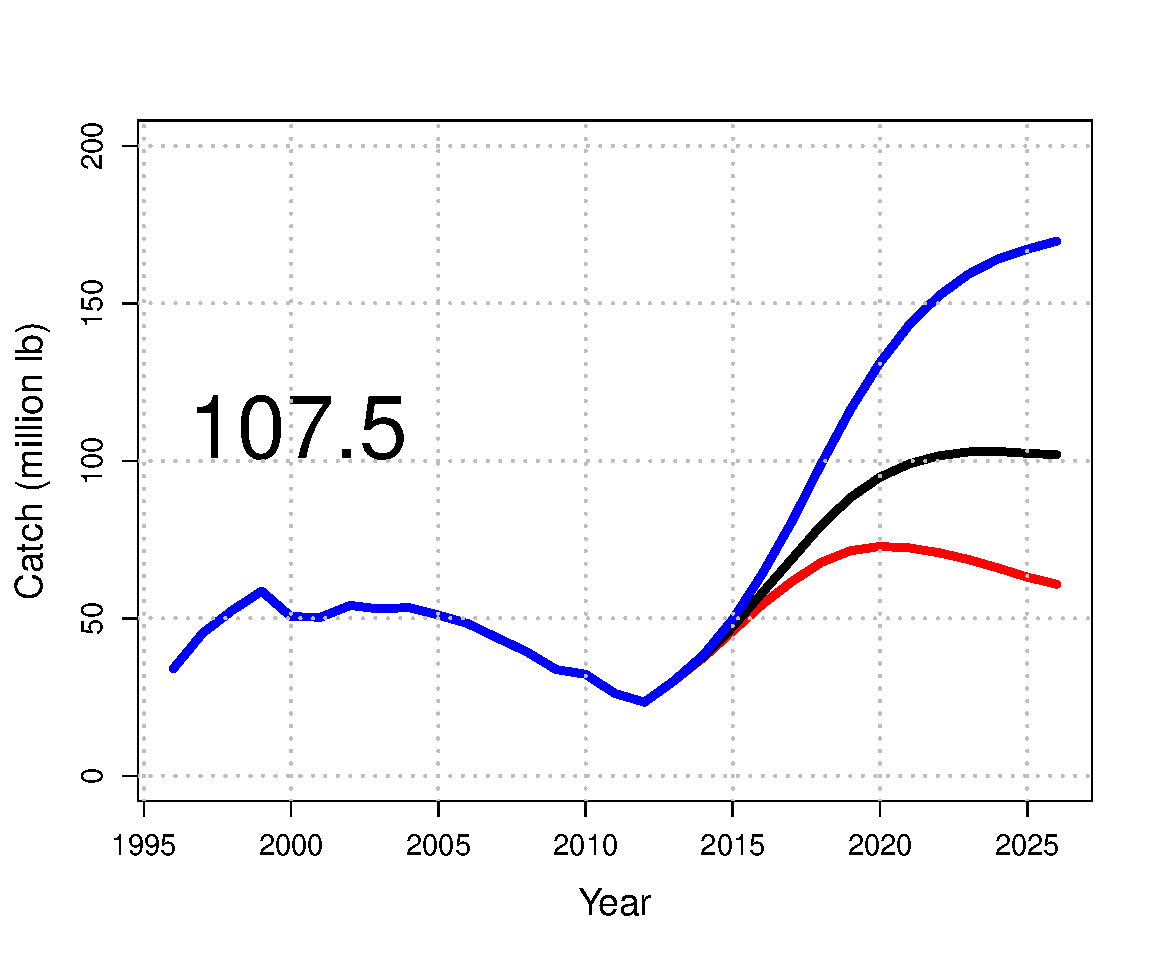
\includegraphics[height=1.5in]{../FIGURES/SIZELIMIT/fig_32_DI_YBio.pdf}
		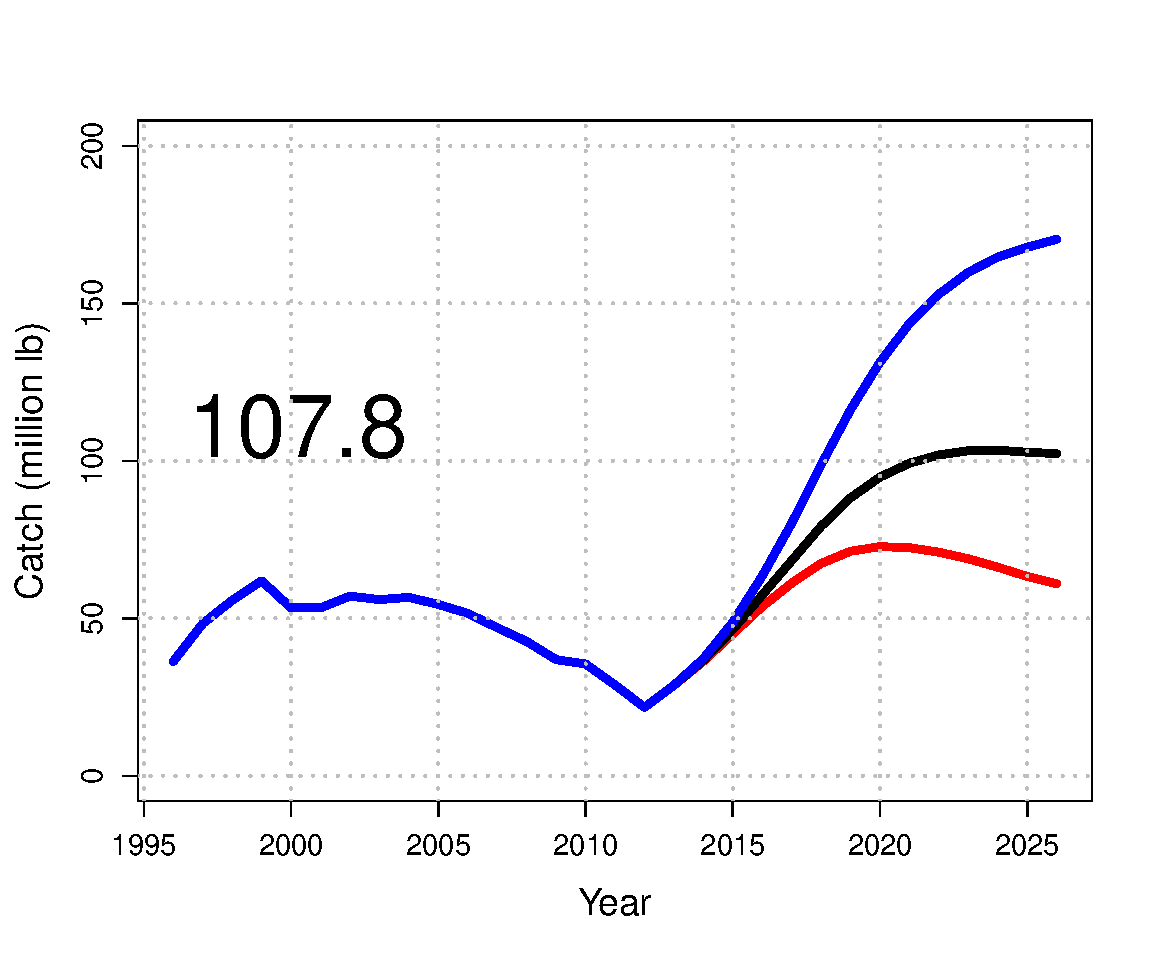
\includegraphics[height=1.5in]{../FIGURES/SIZELIMIT/fig_29_DI_YBio.pdf}
		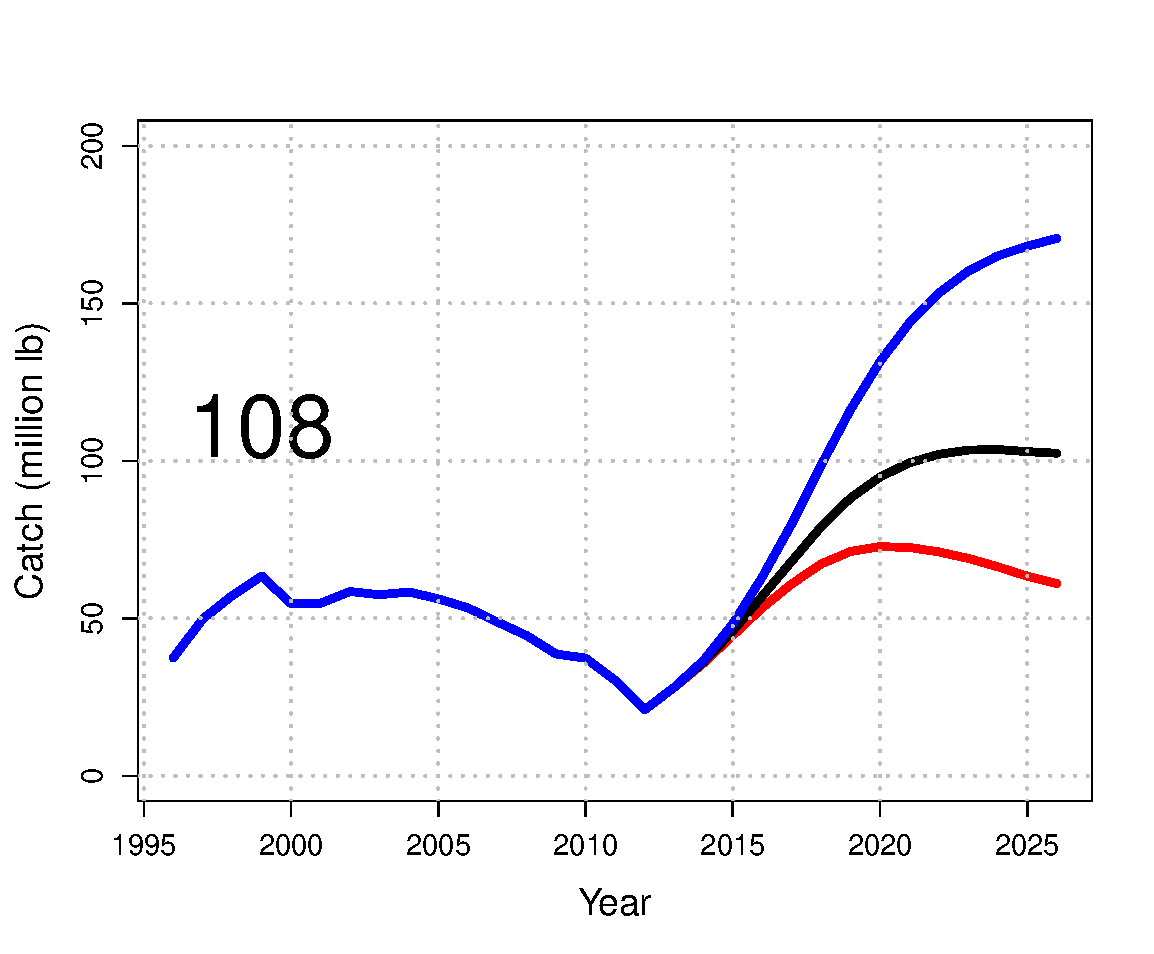
\includegraphics[height=1.5in]{../FIGURES/SIZELIMIT/fig_26_DI_YBio.pdf}
		                                                              
		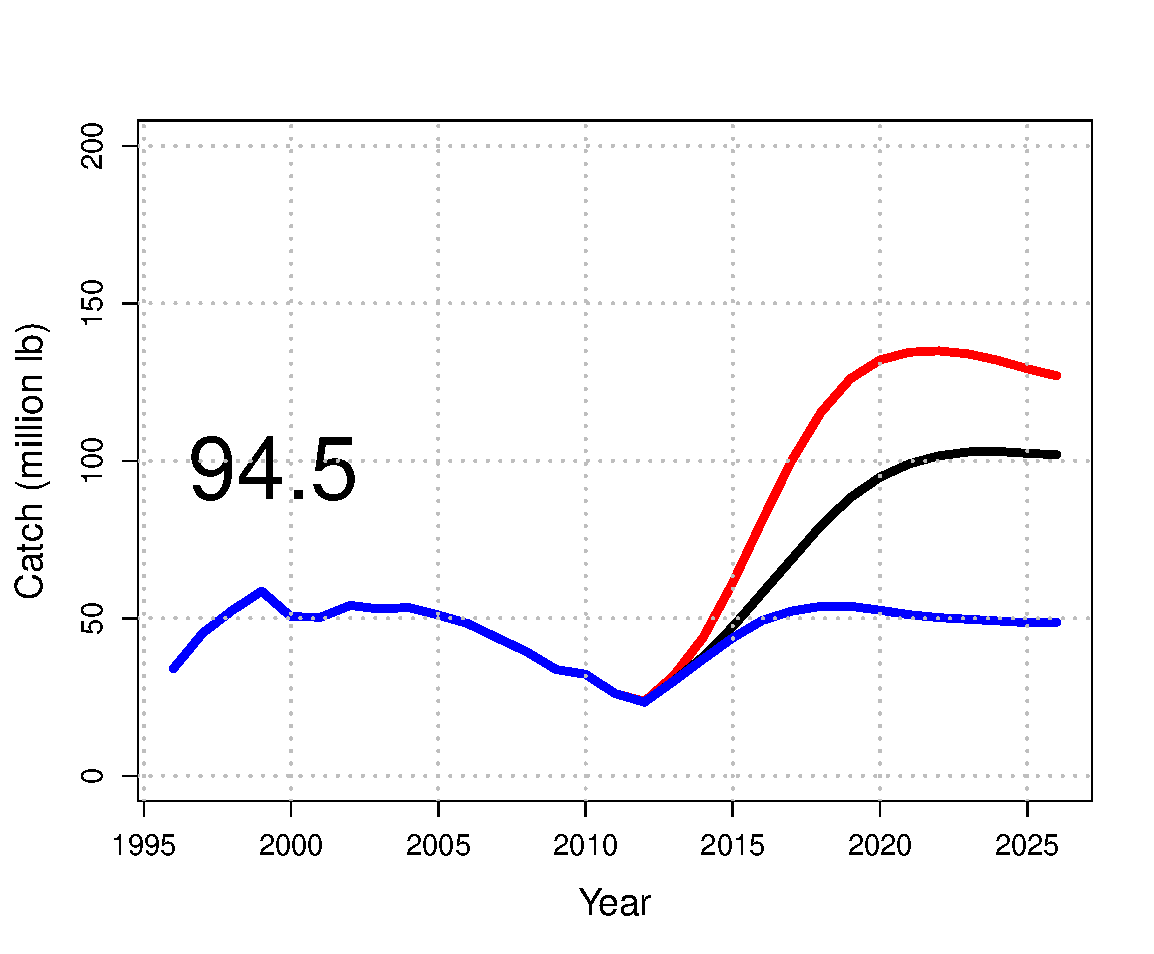
\includegraphics[height=1.5in]{../FIGURES/SIZELIMIT/fig_32_DD_YBio.pdf}
		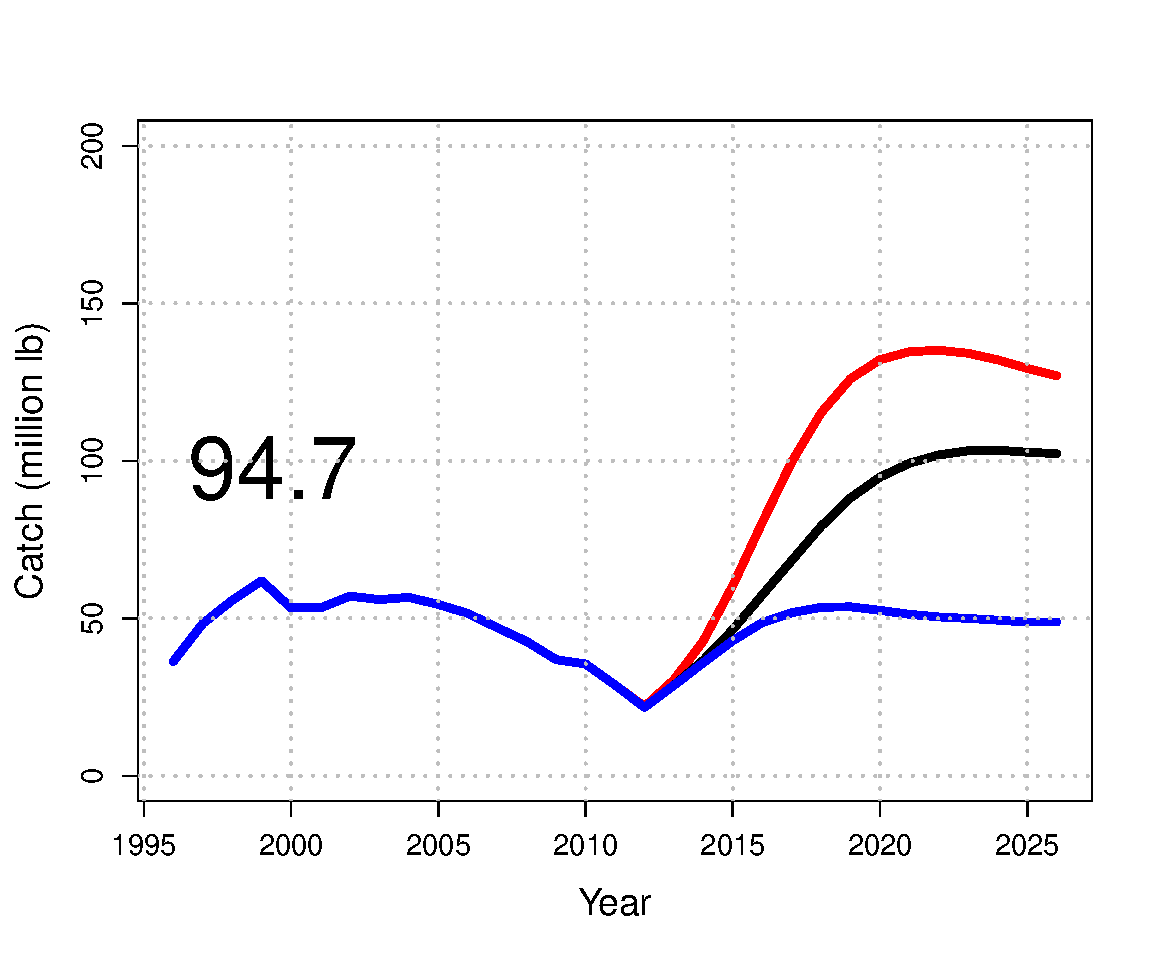
\includegraphics[height=1.5in]{../FIGURES/SIZELIMIT/fig_29_DD_YBio.pdf}
		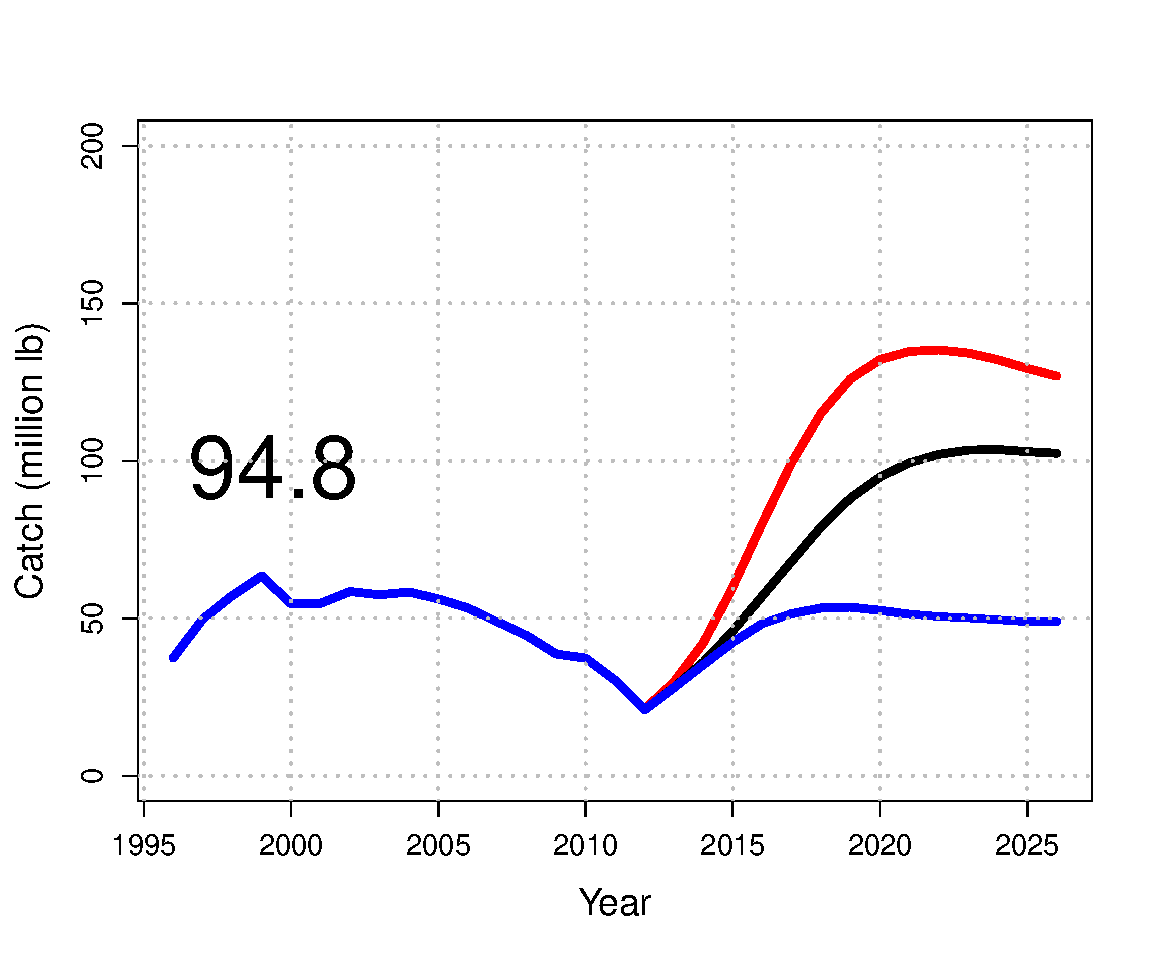
\includegraphics[height=1.5in]{../FIGURES/SIZELIMIT/fig_26_DD_YBio.pdf}
	\caption{Effects of MSL on commercial yield under the assumptions of density-independent growth (top row) and density-dependent growth (bottom row) for 32 inch (left), 29 inch (middle), and 26 inch (right) size limits.  Poor, average, and good recruitment are denoted by red, black and blue lines, respectively.  Value on each panel corresponds to 2020-2025 average over 3 recruitment hypotheses.}
	\label{fig:FIGURES_SIZELIMIT_fig_32_DI_YBio}
\end{figure}
% subsection impacts_of_msl_on_commercial_yield (end)

\subsection{Impacts of MSL on commercial wastage} % (fold)
\label{sub:impacts_of_msl_on_commercial_wastage}

Substantial reductions in commercial wastage occur with a reduction in the minimum size limit.  Under a 32 inch size limit, simulated wastage between 2020 and 20205 averaged 2.494 million pounds and this declined by nearly 90\% to 0.26 million pounds under a 26 inch size limit (Figure \ref{fig:FIGURES_SIZELIMIT_fig_32_DI_WBio}).  Reductions in wastage could also translate into reduced operation costs, as fewer fish have to be captured and discarded to make up the individual vessel quota.  Between the years 2020--2025 and estimated 60\% of the halibut captured in the commercial fishery (assuming a fixed length-based selectivity) are of sublegal size and discarded (Figure \ref{fig:FIGURES_SIZELIMIT_fig_32_DI_dt}).  Reducing the size limit from 32 inches to 29 or 26 inches would reduce this fraction to 30\% and 10\%, respectively.  Reducing the size limit from 32 to 26 inches increases the overall retention probability from 40\% to 90\%.  

\begin{figure}[htbp]
	\centering
		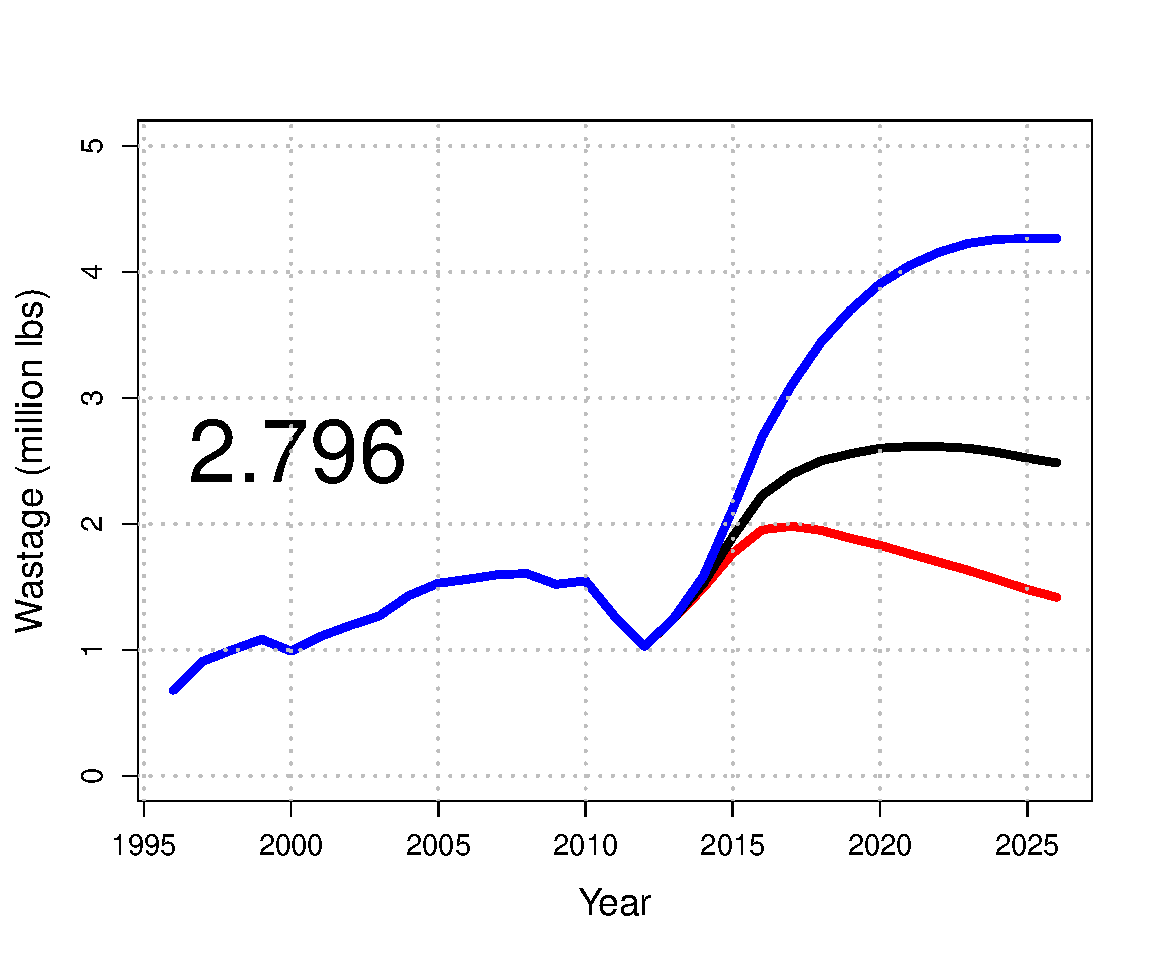
\includegraphics[height=1.5in]{../FIGURES/SIZELIMIT/fig_32_DI_WBio.pdf}
		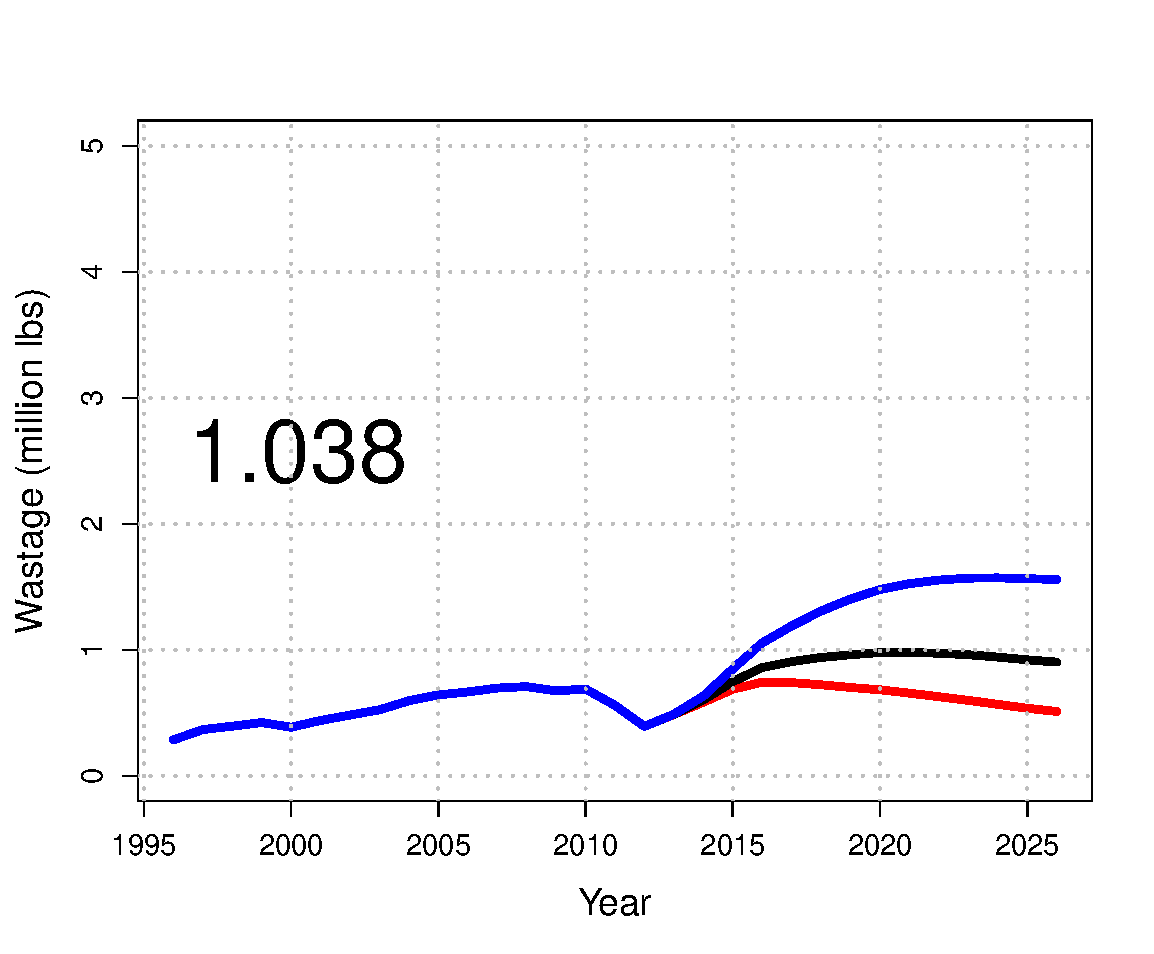
\includegraphics[height=1.5in]{../FIGURES/SIZELIMIT/fig_29_DI_WBio.pdf}
		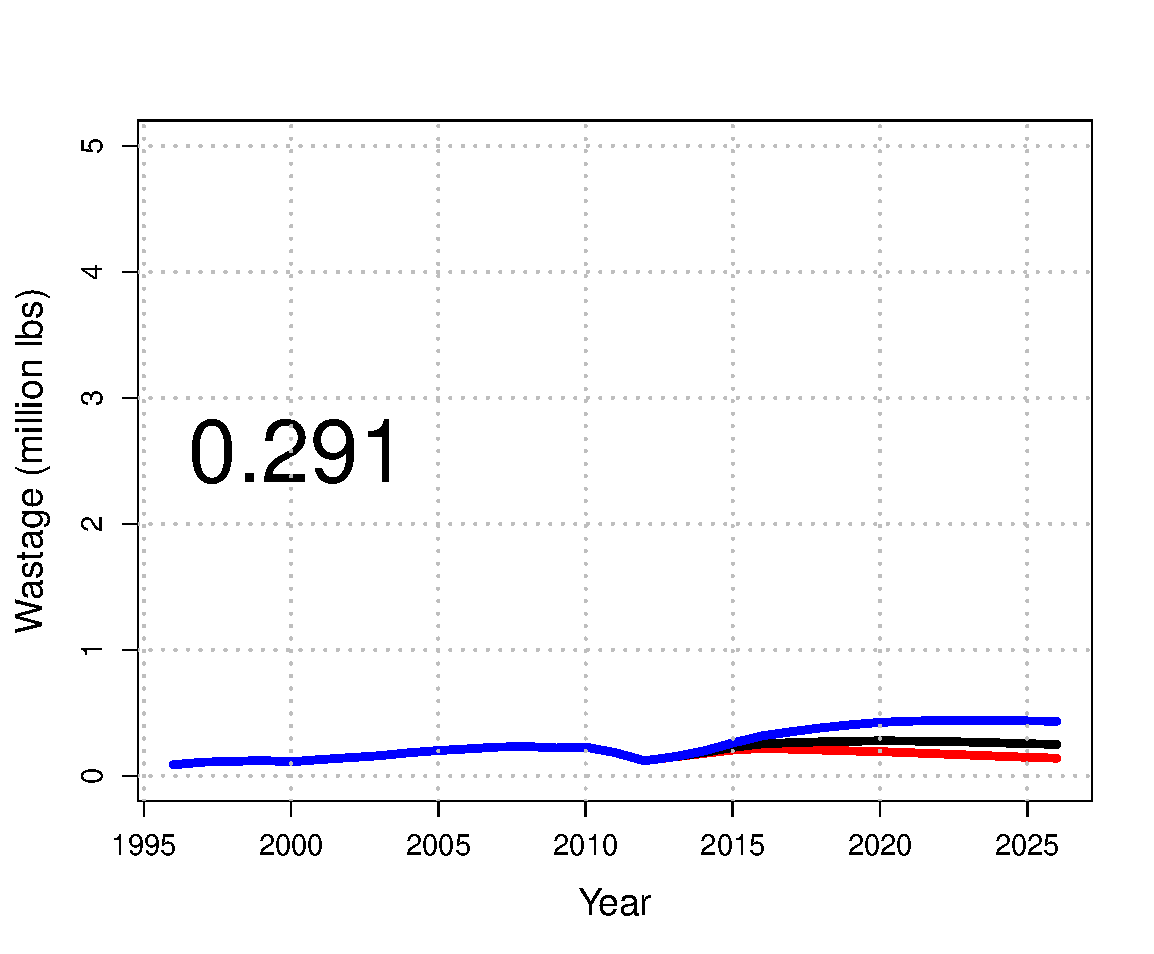
\includegraphics[height=1.5in]{../FIGURES/SIZELIMIT/fig_26_DI_WBio.pdf}
		                                                              
		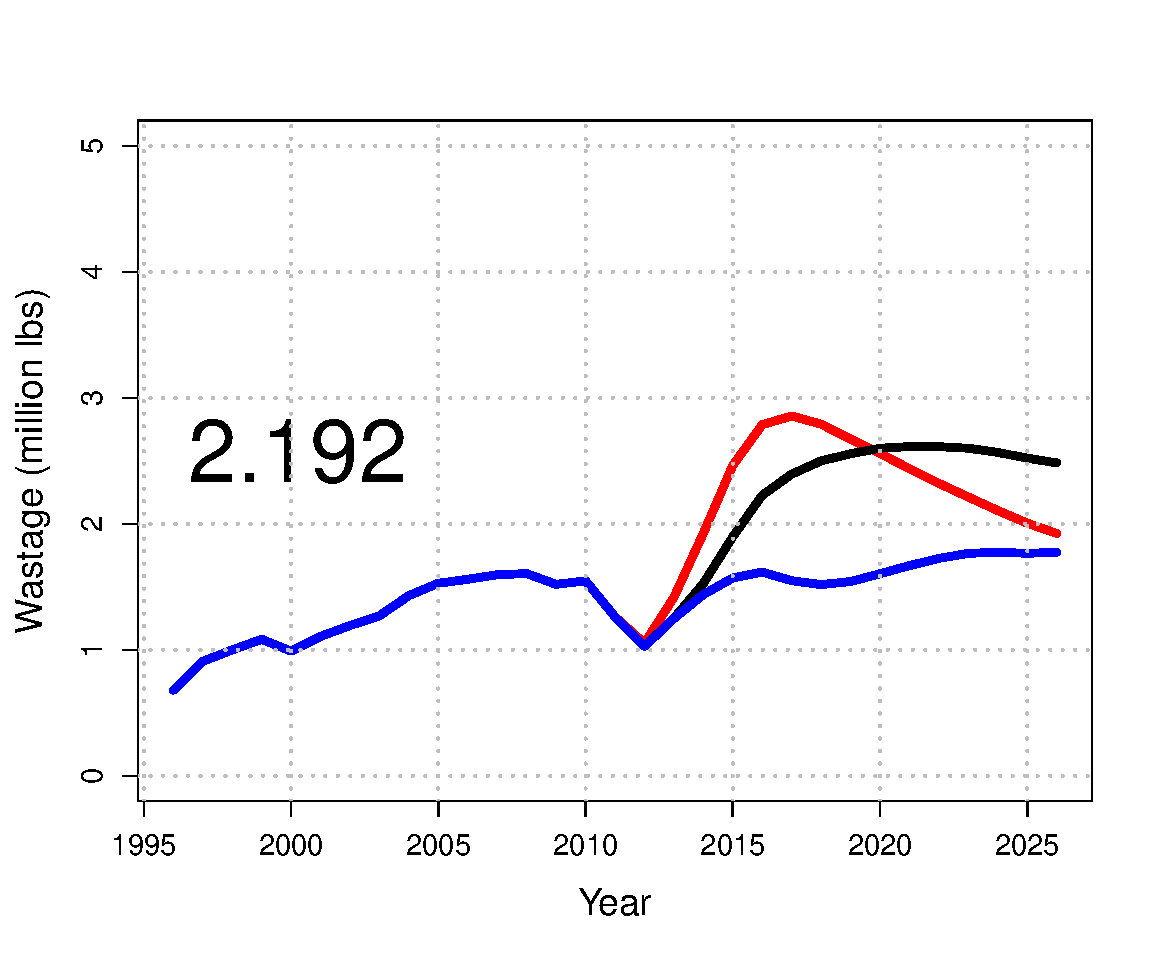
\includegraphics[height=1.5in]{../FIGURES/SIZELIMIT/fig_32_DD_WBio.pdf}
		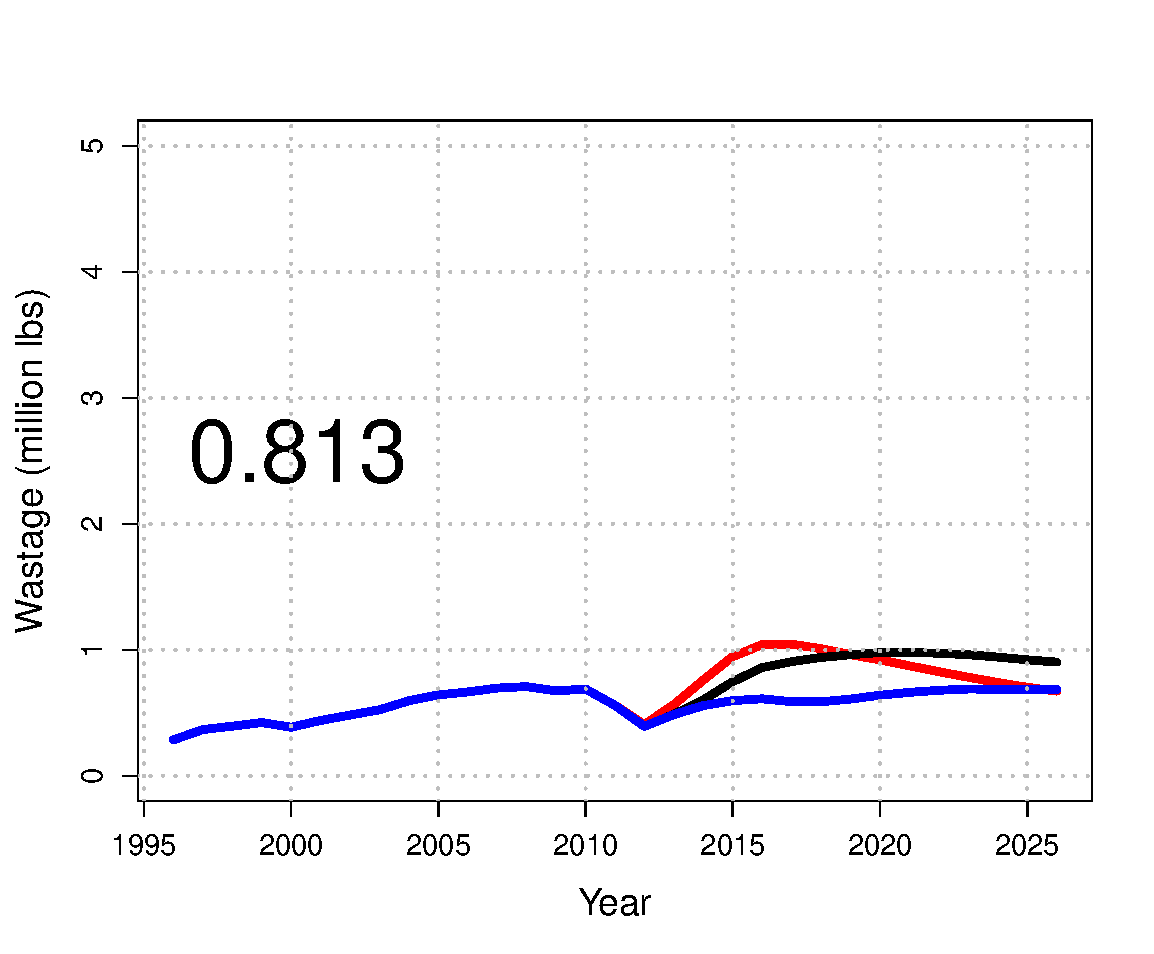
\includegraphics[height=1.5in]{../FIGURES/SIZELIMIT/fig_29_DD_WBio.pdf}
		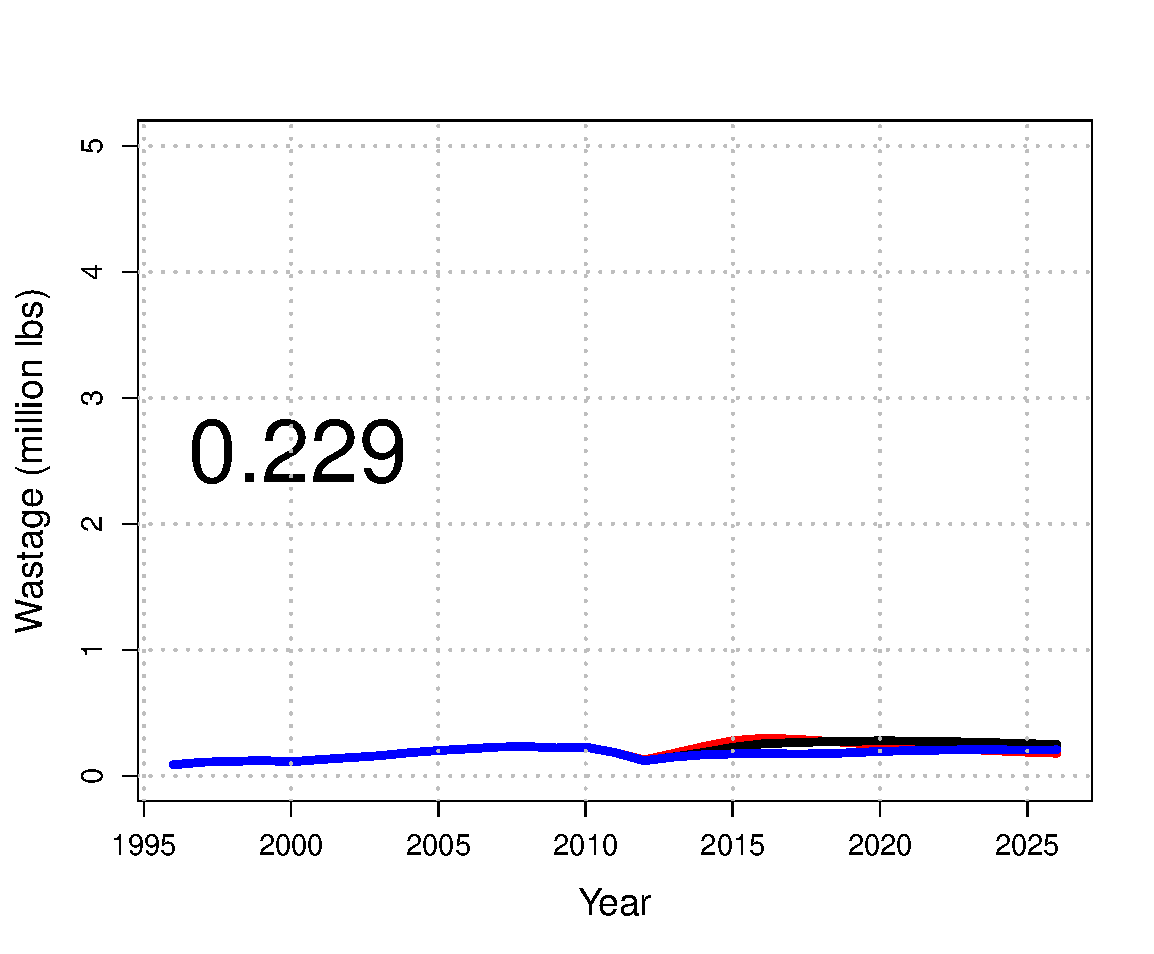
\includegraphics[height=1.5in]{../FIGURES/SIZELIMIT/fig_26_DD_WBio.pdf}
	\caption{Effects of MSL on commercial wastage under the assumptions of density-independent growth (top row) and density-dependent growth (bottom row) for 32 inch (left), 29 inch (middle), and 26 inch (right) size limits.  Poor, average, and good recruitment are denoted by red, black and blue lines, respectively.  Value on each panel corresponds to 2020-2025 average over 3 recruitment hypotheses.}
	\label{fig:FIGURES_SIZELIMIT_fig_32_DI_WBio}
\end{figure}

\begin{figure}[htbp]
	\centering
		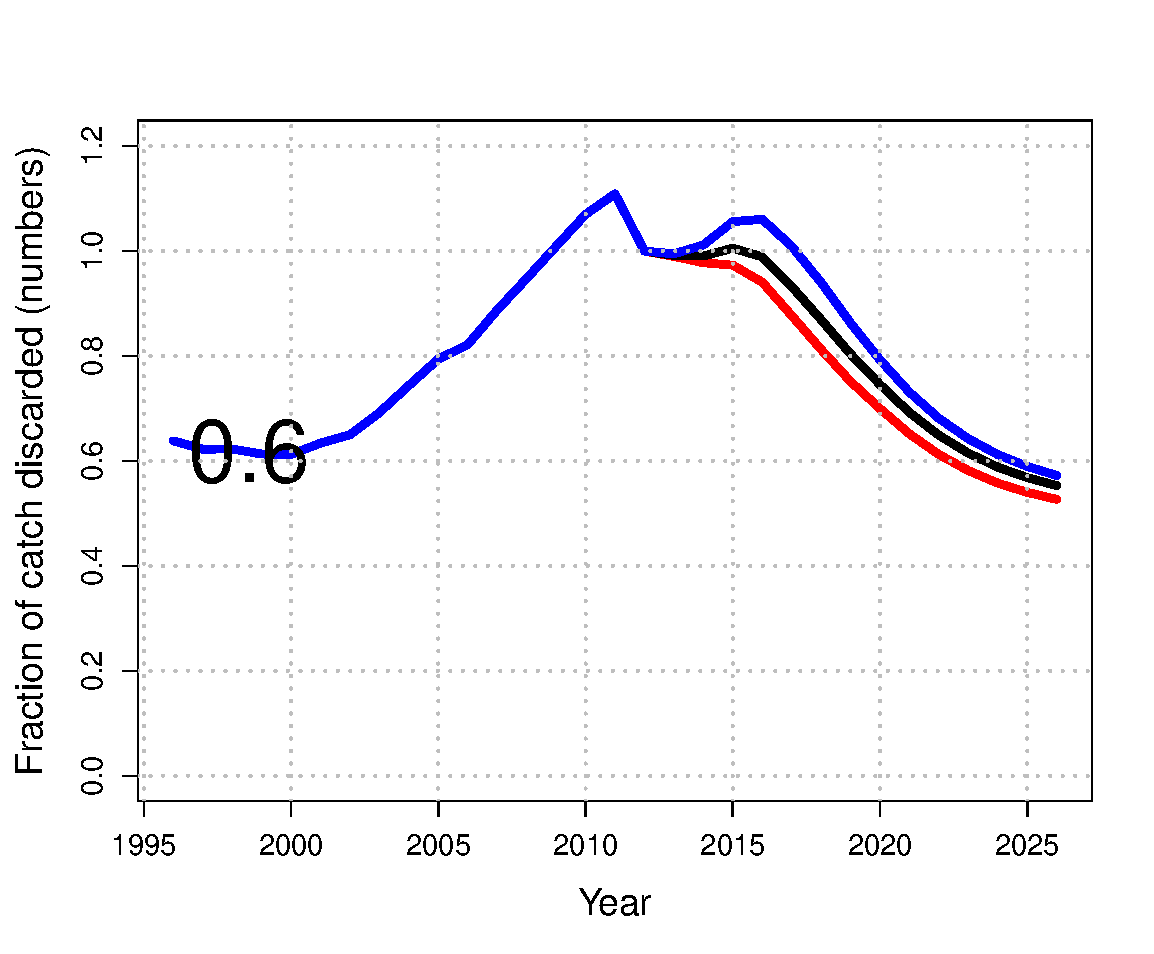
\includegraphics[height=1.5in]{../FIGURES/SIZELIMIT/fig_32_DI_dt.pdf}
		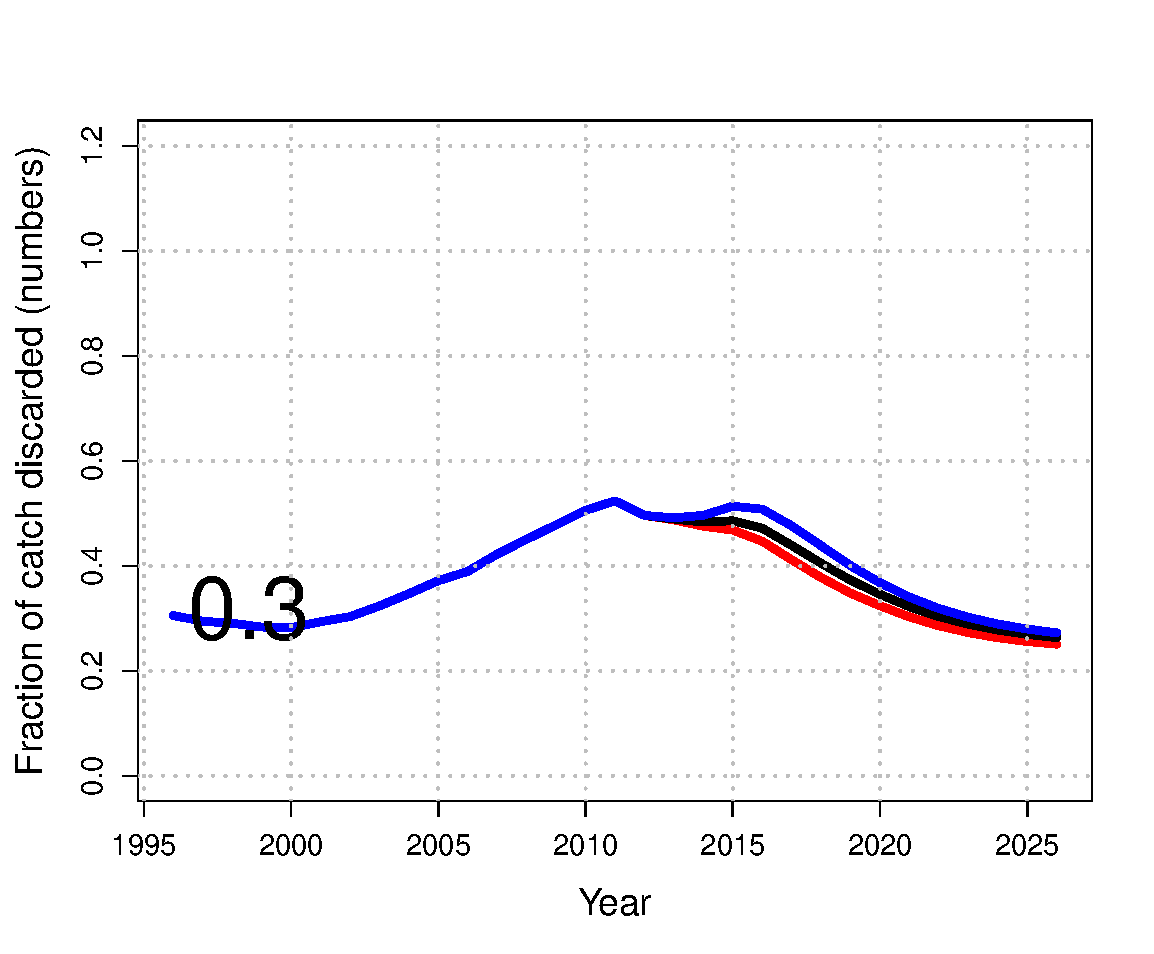
\includegraphics[height=1.5in]{../FIGURES/SIZELIMIT/fig_29_DI_dt.pdf}
		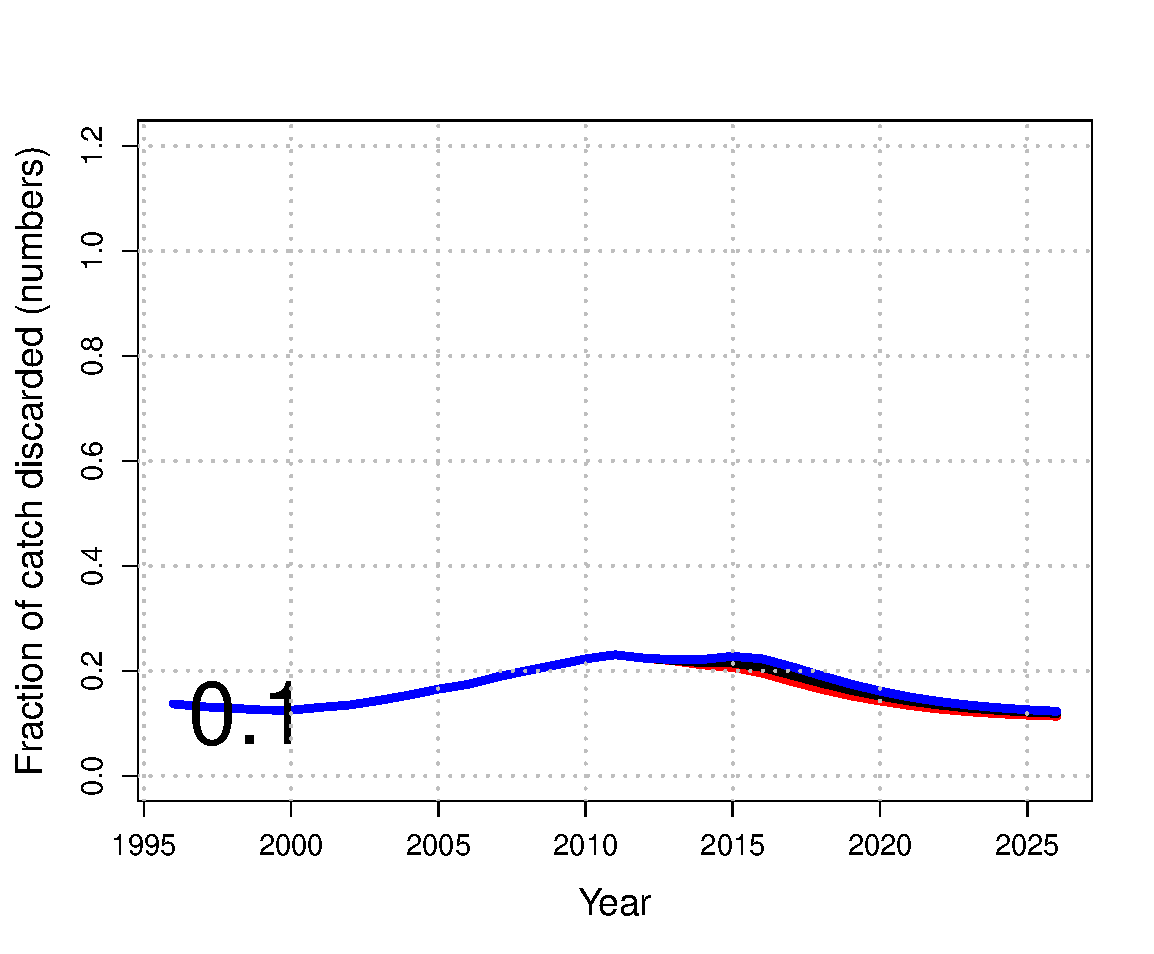
\includegraphics[height=1.5in]{../FIGURES/SIZELIMIT/fig_26_DI_dt.pdf}
		                                                              
		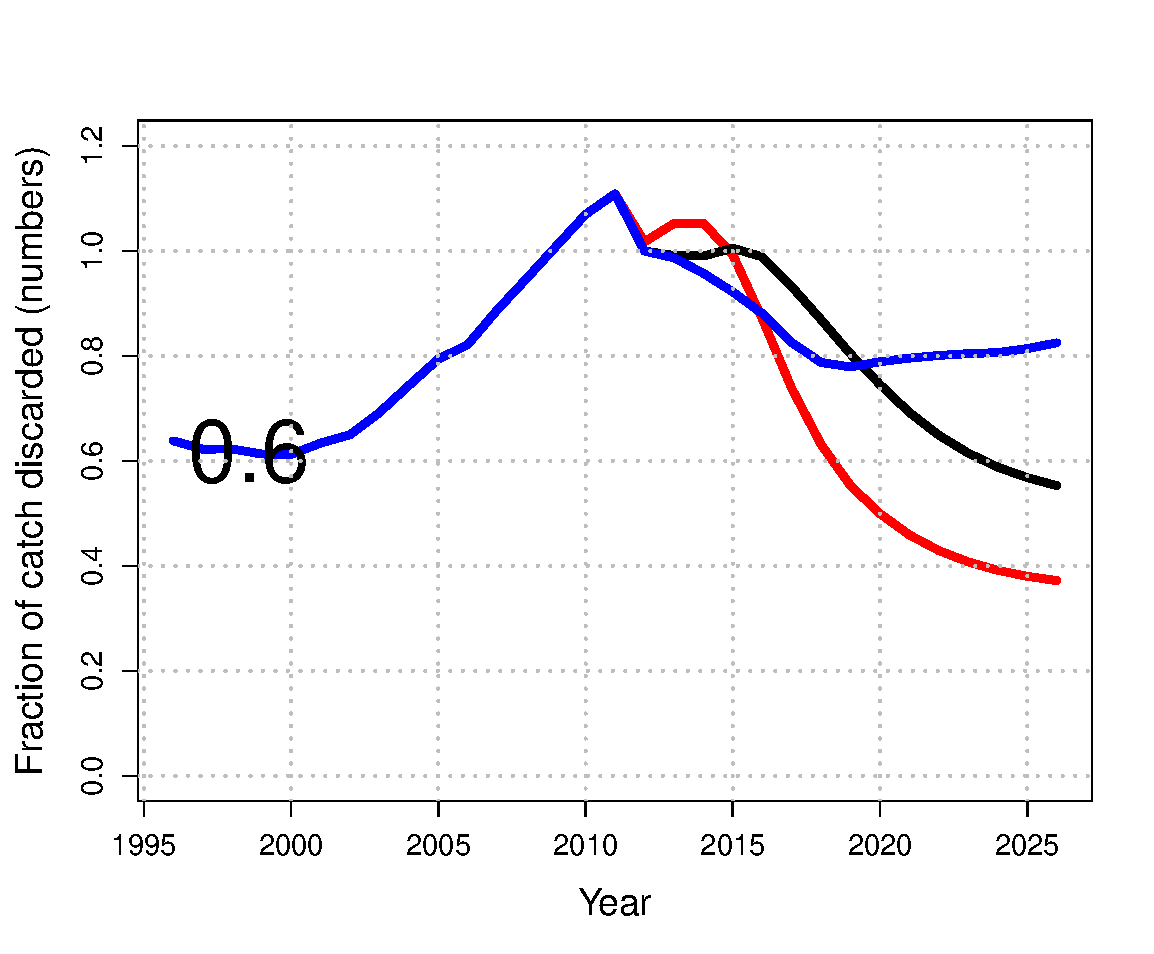
\includegraphics[height=1.5in]{../FIGURES/SIZELIMIT/fig_32_DD_dt.pdf}
		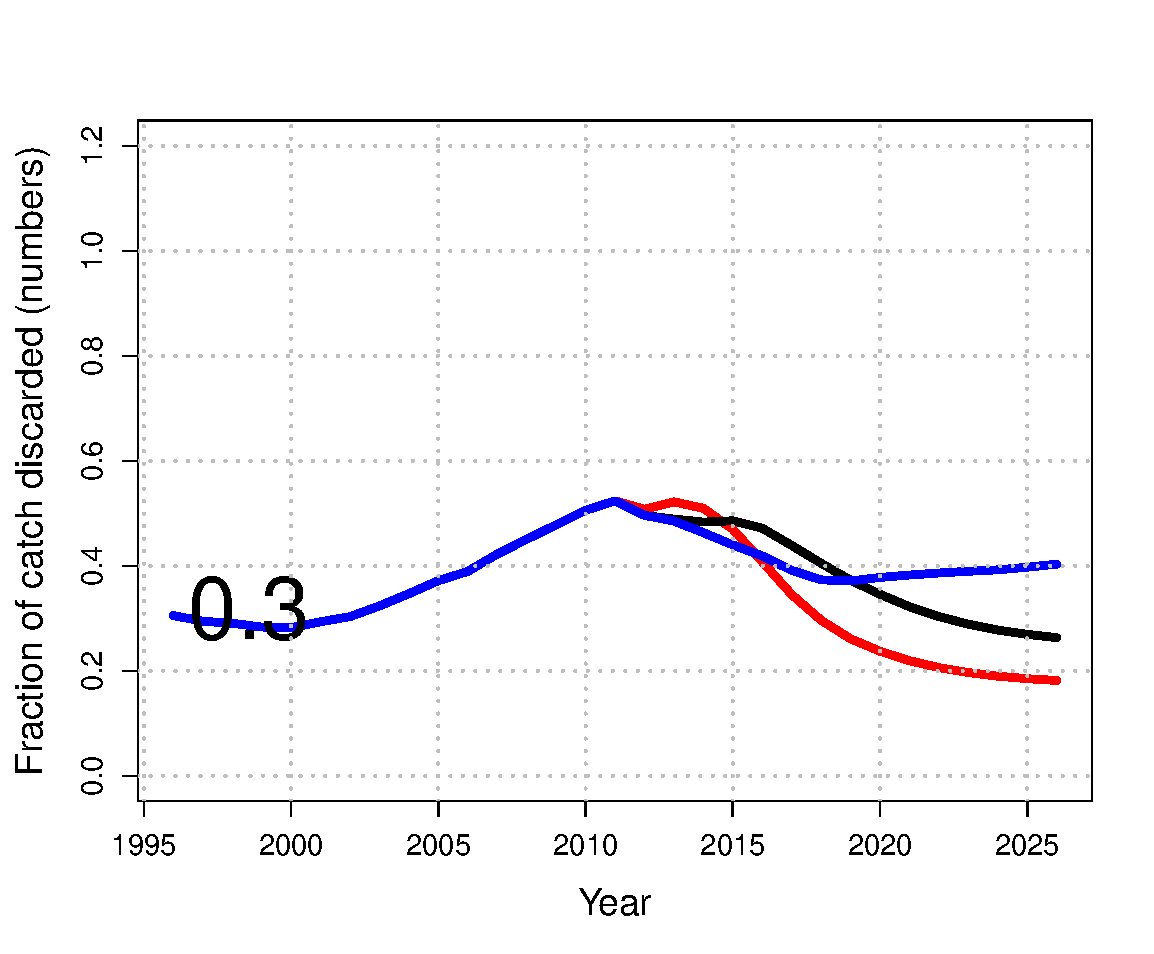
\includegraphics[height=1.5in]{../FIGURES/SIZELIMIT/fig_29_DD_dt.pdf}
		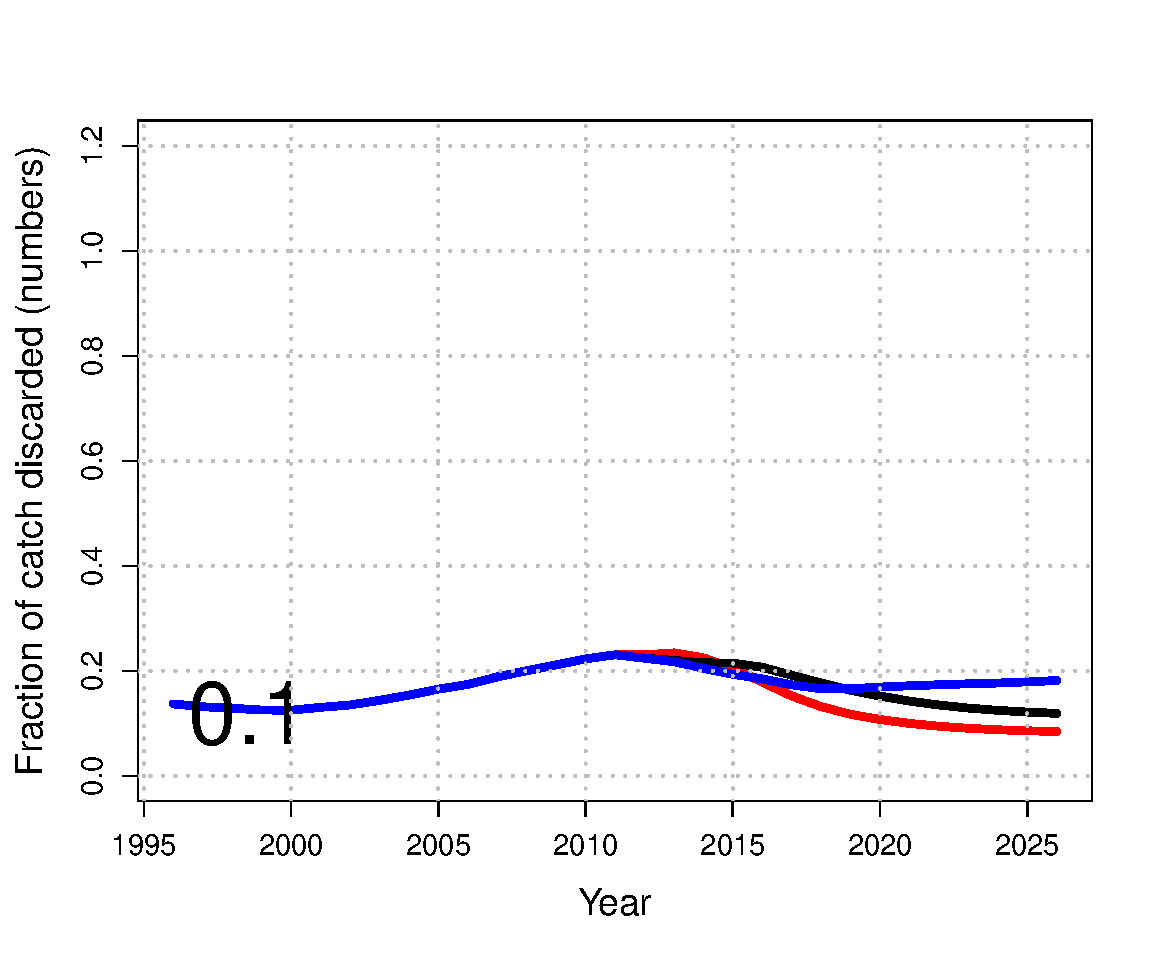
\includegraphics[height=1.5in]{../FIGURES/SIZELIMIT/fig_26_DD_dt.pdf}
	\caption{Fraction of captured fish discarded in the commercial fishery under the assumptions of density-independent growth (top row) and density-dependent growth (bottom row) for 32 inch (left), 29 inch (middle), and 26 inch (right) size limits.  Poor, average, and good recruitment are denoted by red, black and blue lines, respectively.  Value on each panel corresponds to 2020-2025 average over 3 recruitment hypotheses.}
	\label{fig:FIGURES_SIZELIMIT_fig_32_DI_dt}
\end{figure}

% subsection impacts_of_msl_on_commercial_wastage (end)

\subsection{Impacts of MSL on economic value} % (fold)
\label{sub:impacts_of_msl_on_economic_value}

Decreasing the MLS to smaller sizes reduces the overall landed value of the commercial fishery because the composition of the catch contains a higher fraction of lower value 5-10 pound fish (assuming \$5.00 per pound).  The simulated projected landed value between 2020--2025 decreases from \$684.7 million to \$683 million  (or \$1.7 million) with a change in MLS of 32 inches to 26 inches (Figure \ref{fig:FIGURES_SIZELIMIT_fig_32_DI_LVal}).

Based on the allometric length-weight relationship a 26 inch halibut is roughly 5 pounds net weight, and a 32 inch halibut is roughly 10 pounds net weight. Assuming a price of \$5.00 per pound for halibut in the 5-10 pound range, the potential value of the sub-legal fish that are discarded and assumed to die (with 16\% discard mortality rate) can be calculated.  Under a 32 inch size limit the average value of the wastage is \$15.5 million, and under a 26 inch size limit the value of the wastage is reduced by 90\% to  \$1.55 million (Figure \ref{fig:FIGURES_SIZELIMIT_fig_32_DI_WVal}).  Moreover, the value of this wastage is of dead fish that cannot be recovered in the future.


\begin{figure}[htbp]
	\centering
		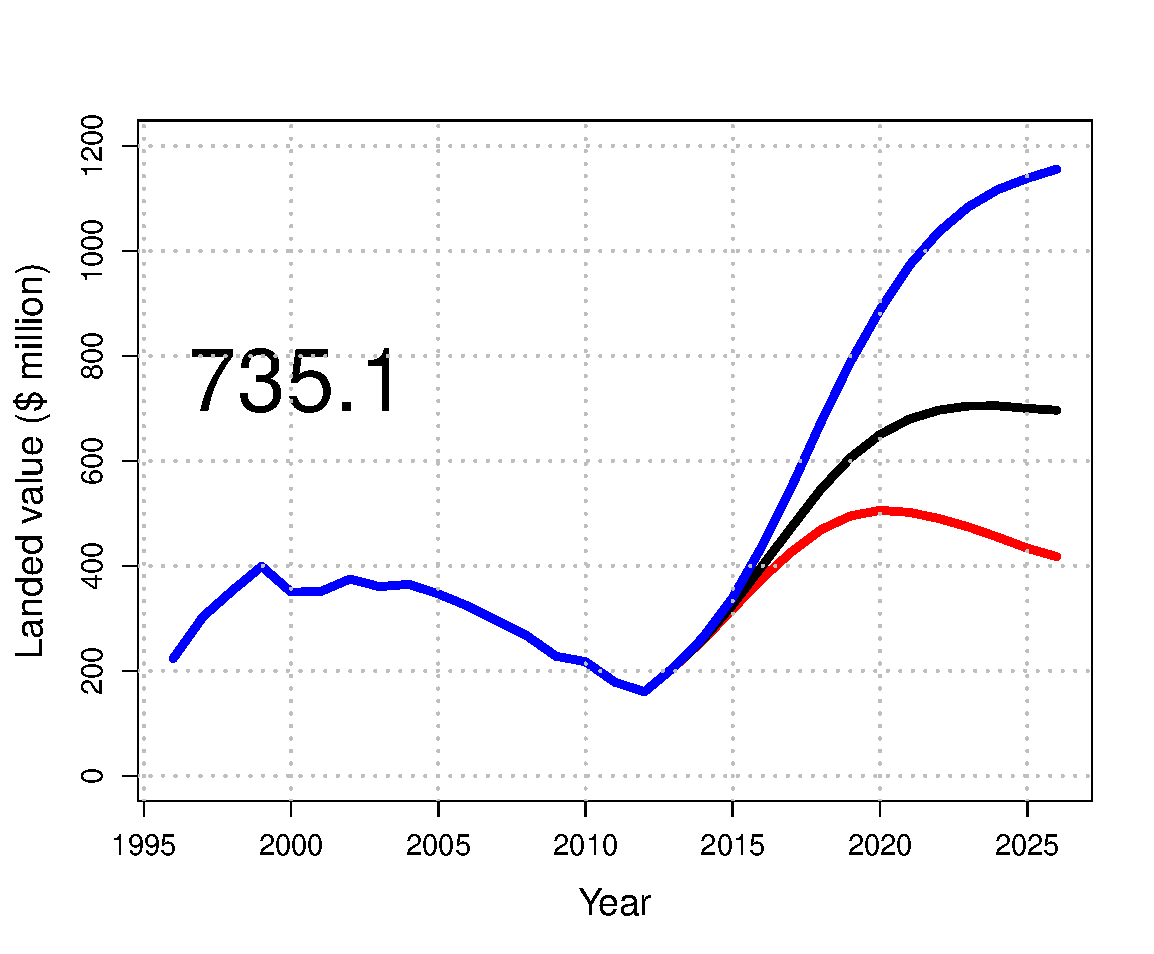
\includegraphics[height=1.5in]{../FIGURES/SIZELIMIT/fig_32_DI_LVal.pdf}
		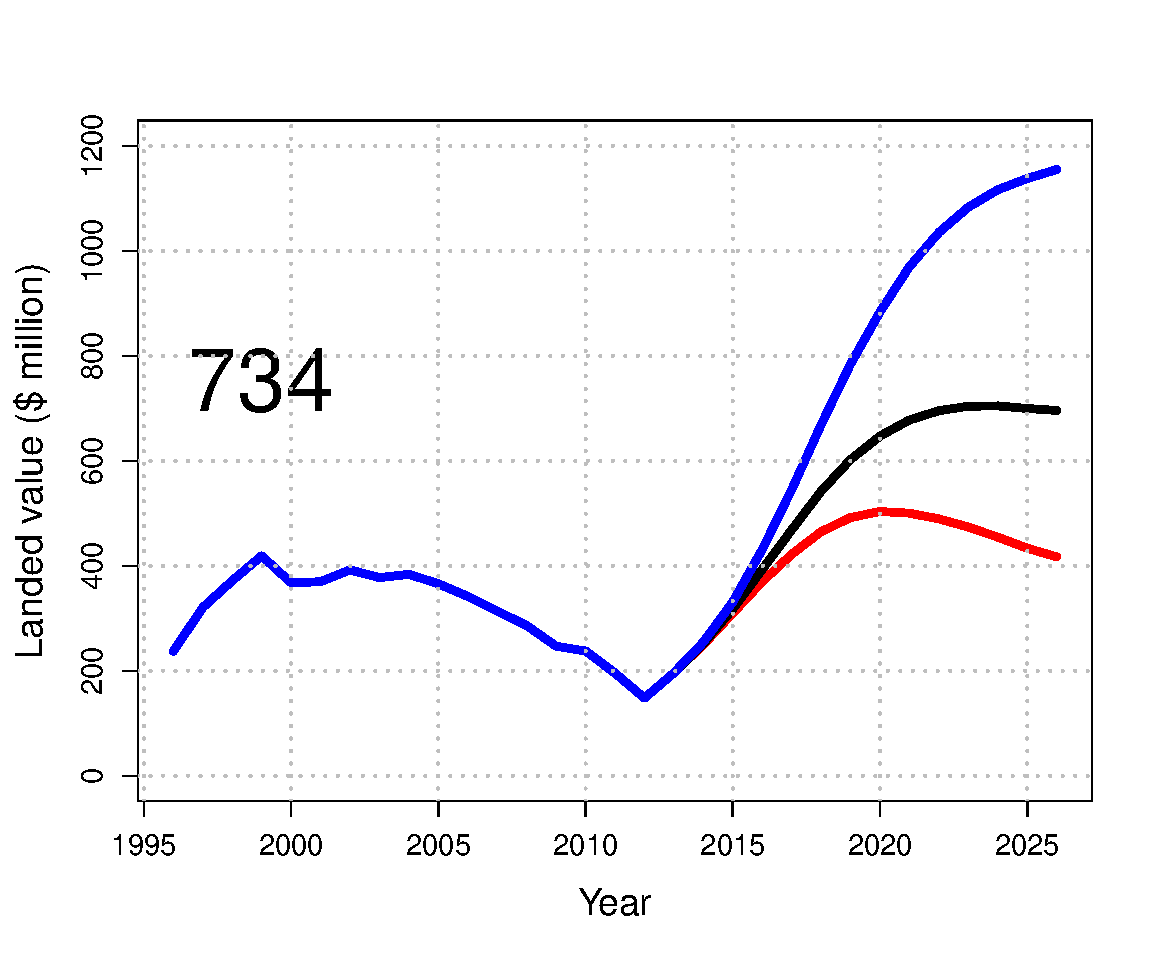
\includegraphics[height=1.5in]{../FIGURES/SIZELIMIT/fig_29_DI_LVal.pdf}
		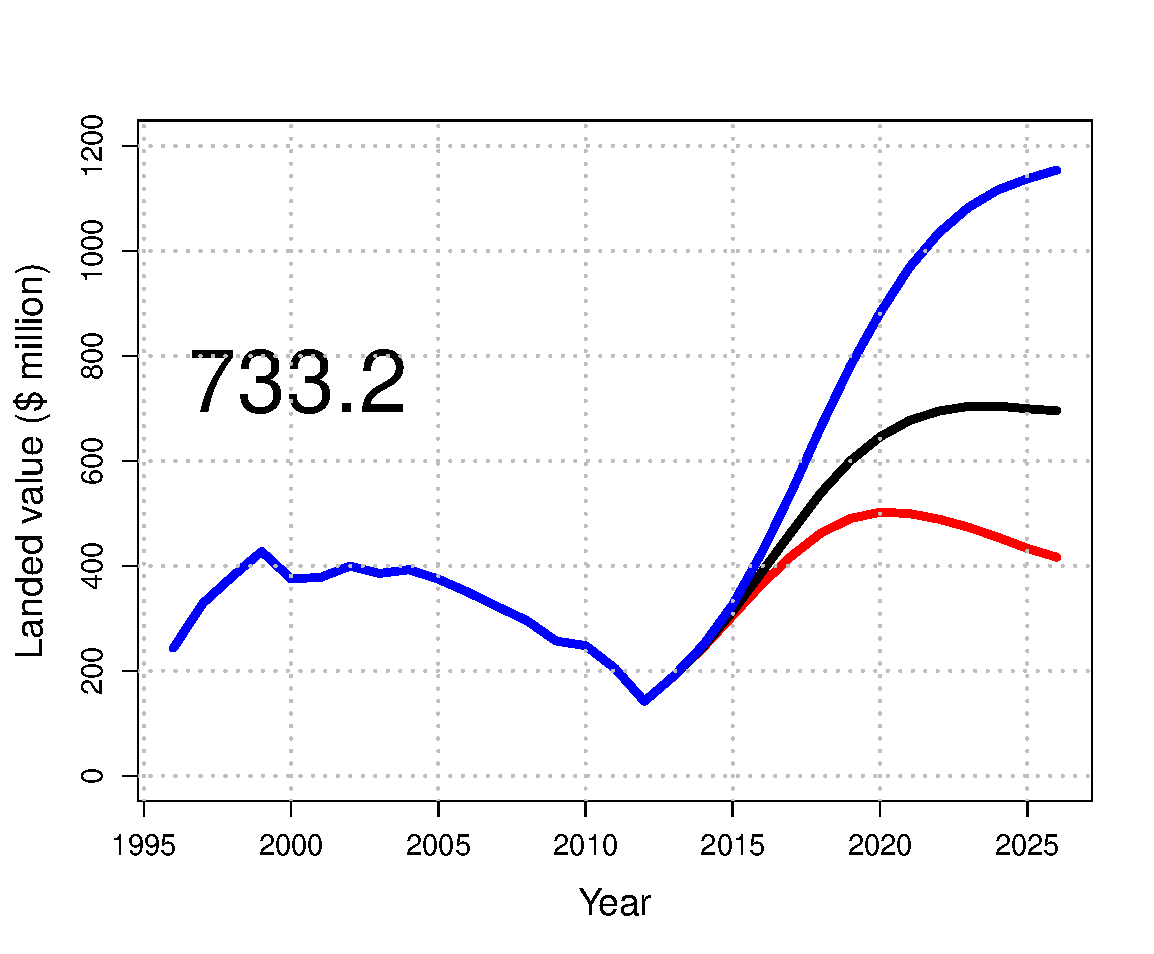
\includegraphics[height=1.5in]{../FIGURES/SIZELIMIT/fig_26_DI_LVal.pdf}
		                                                              
		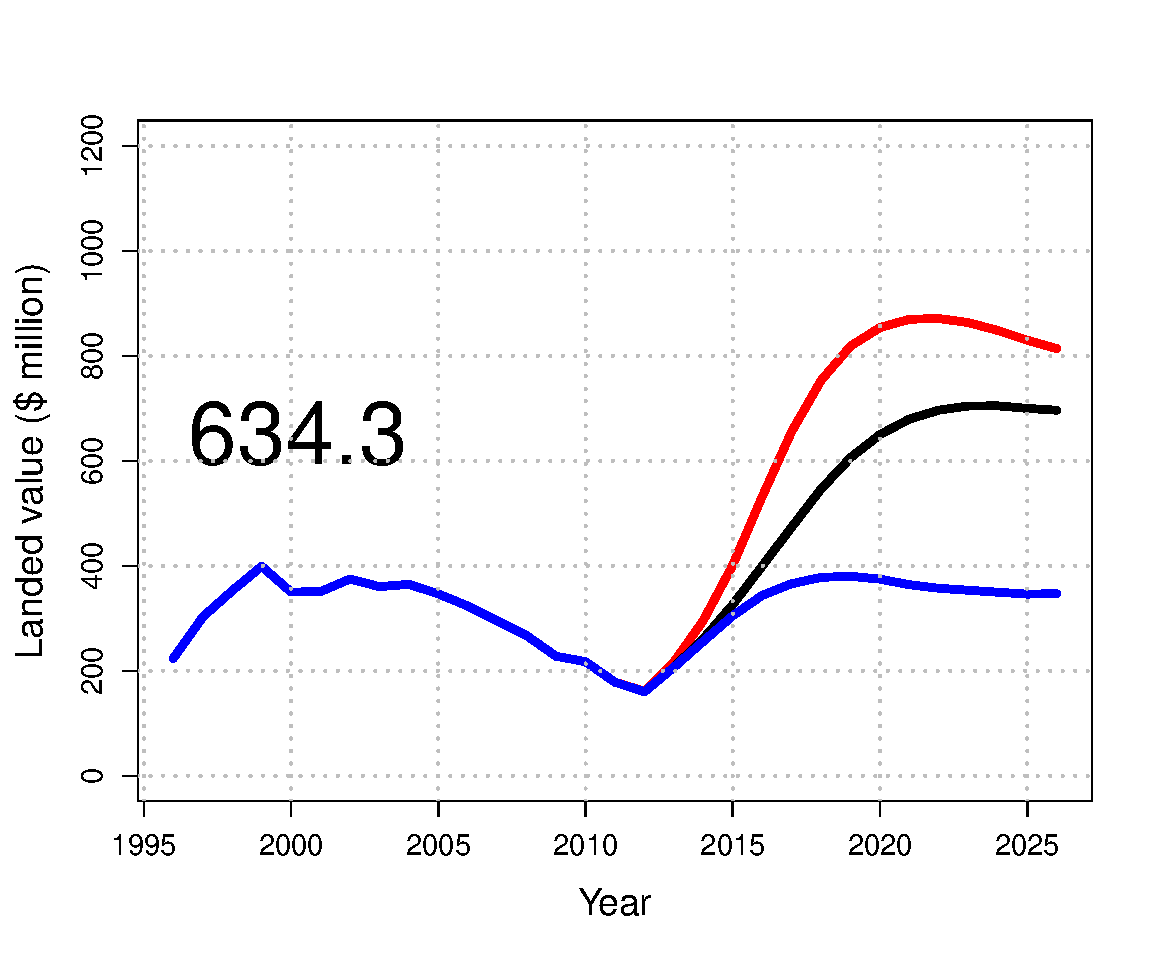
\includegraphics[height=1.5in]{../FIGURES/SIZELIMIT/fig_32_DD_LVal.pdf}
		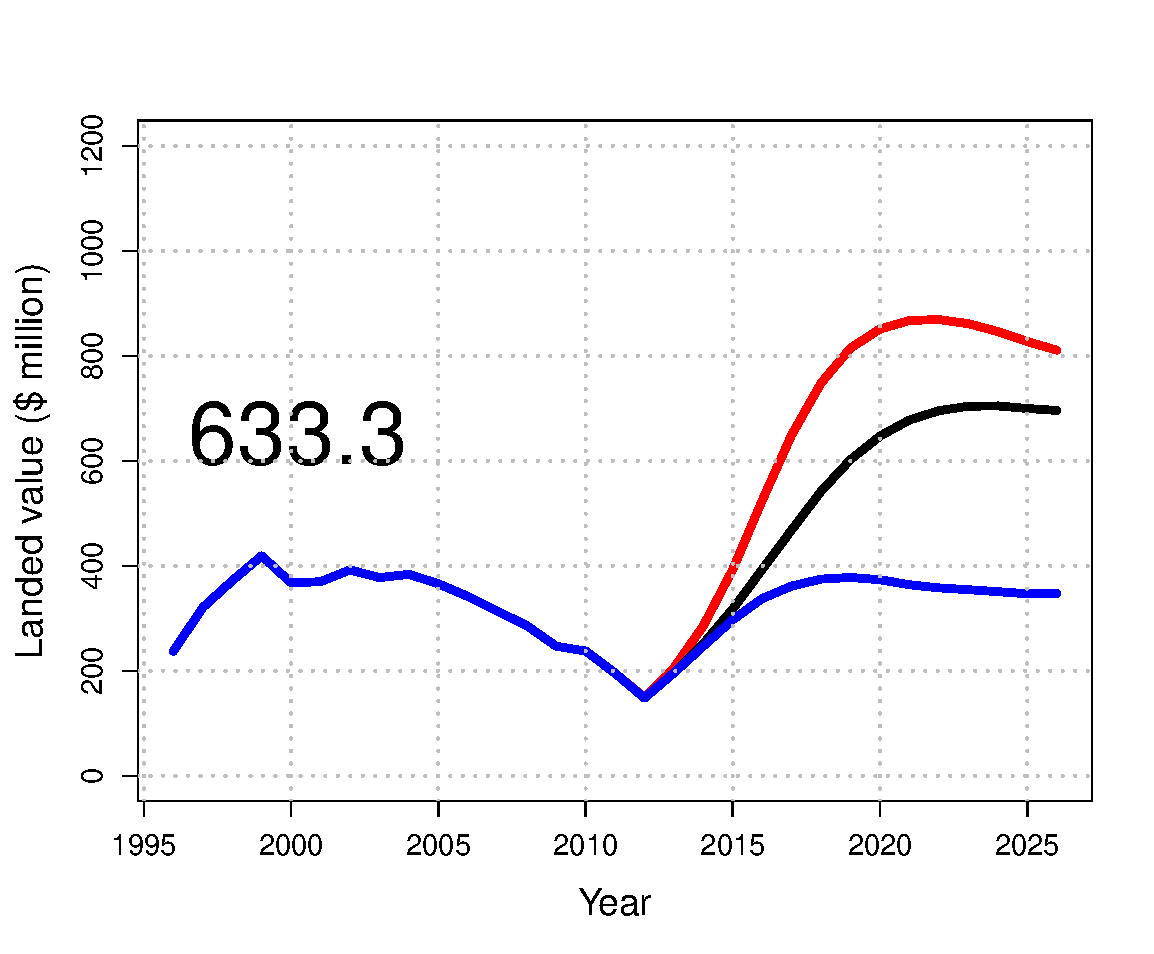
\includegraphics[height=1.5in]{../FIGURES/SIZELIMIT/fig_29_DD_LVal.pdf}
		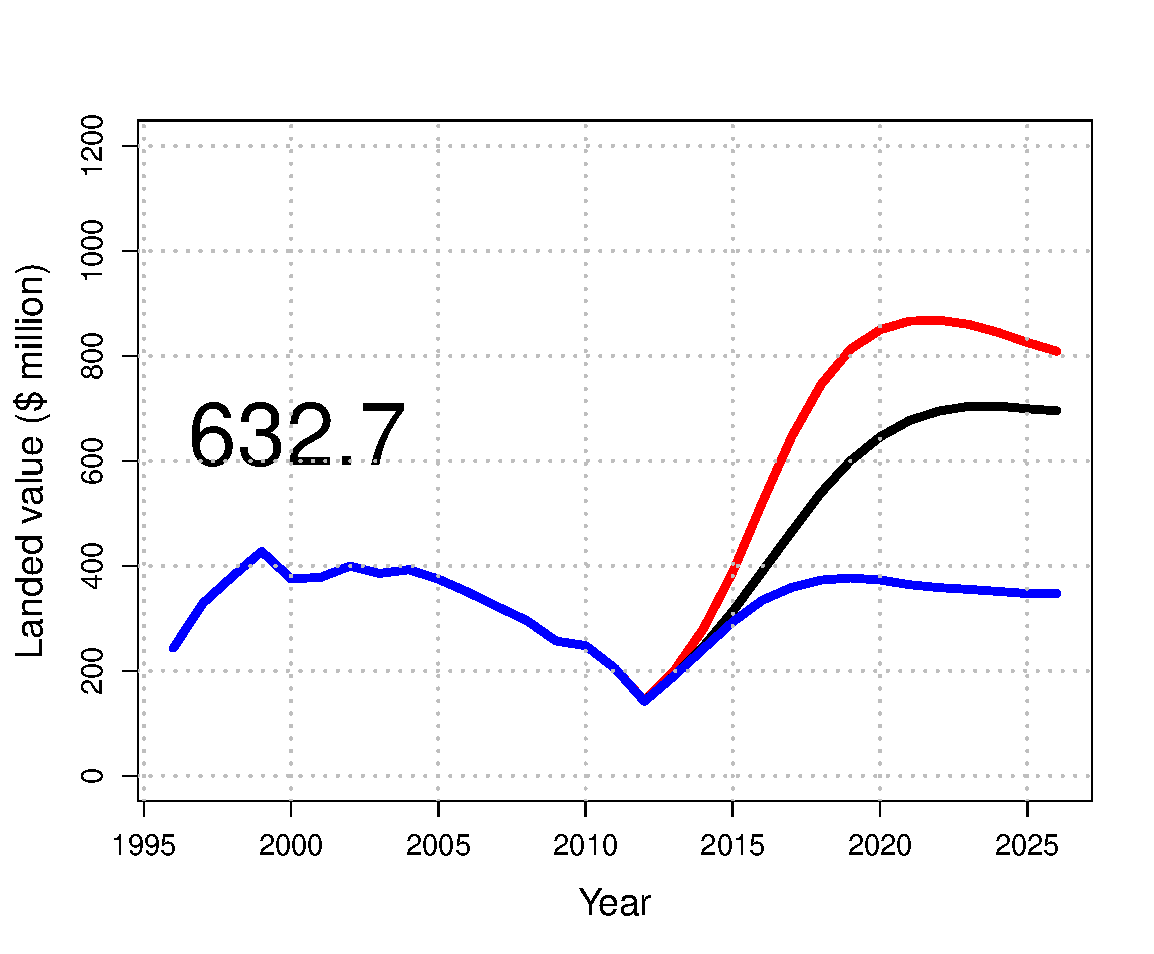
\includegraphics[height=1.5in]{../FIGURES/SIZELIMIT/fig_26_DD_LVal.pdf}
	\caption{Landed value for the commercial fisher under the assumptions of density-independent growth (top row) and density-dependent growth (bottom row) for 32 inch (left), 29 inch (middle), and 26 inch (right) size limits.  Poor, average, and good recruitment are denoted by red, black and blue lines, respectively.  Value on each panel corresponds to 2020-2025 average over 3 recruitment hypotheses.}
	\label{fig:FIGURES_SIZELIMIT_fig_32_DI_LVal}
\end{figure}

\begin{figure}[htbp]
	\centering
		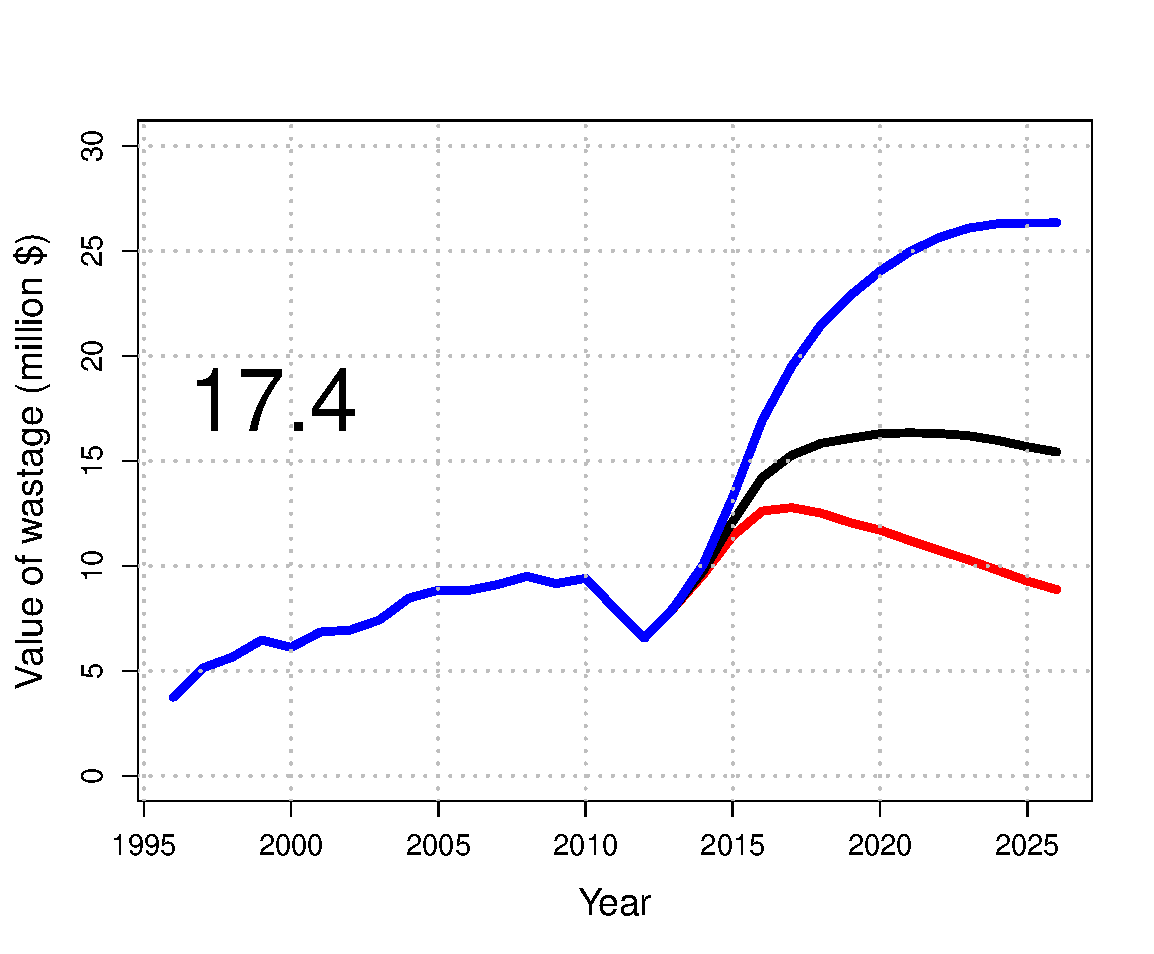
\includegraphics[height=1.5in]{../FIGURES/SIZELIMIT/fig_32_DI_WVal.pdf}
		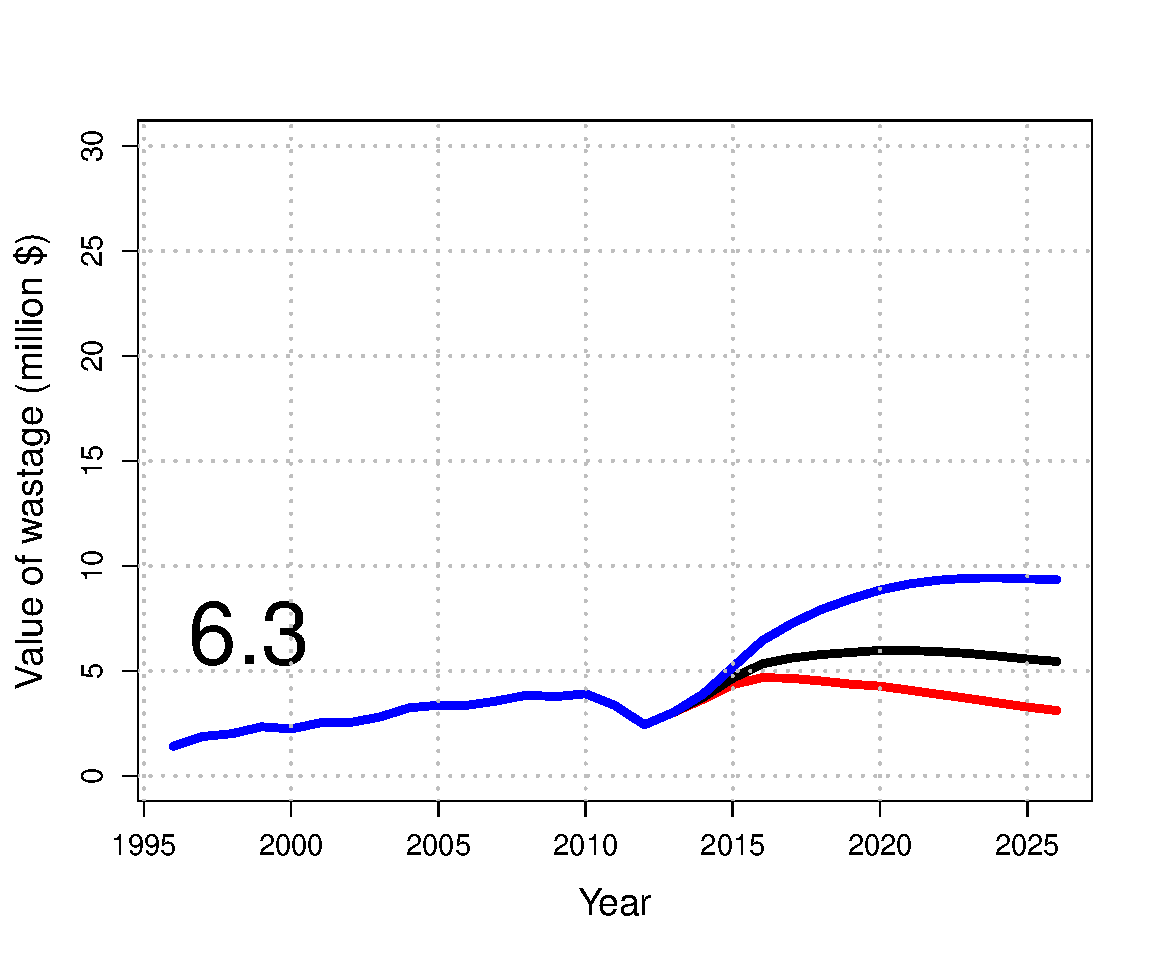
\includegraphics[height=1.5in]{../FIGURES/SIZELIMIT/fig_29_DI_WVal.pdf}
		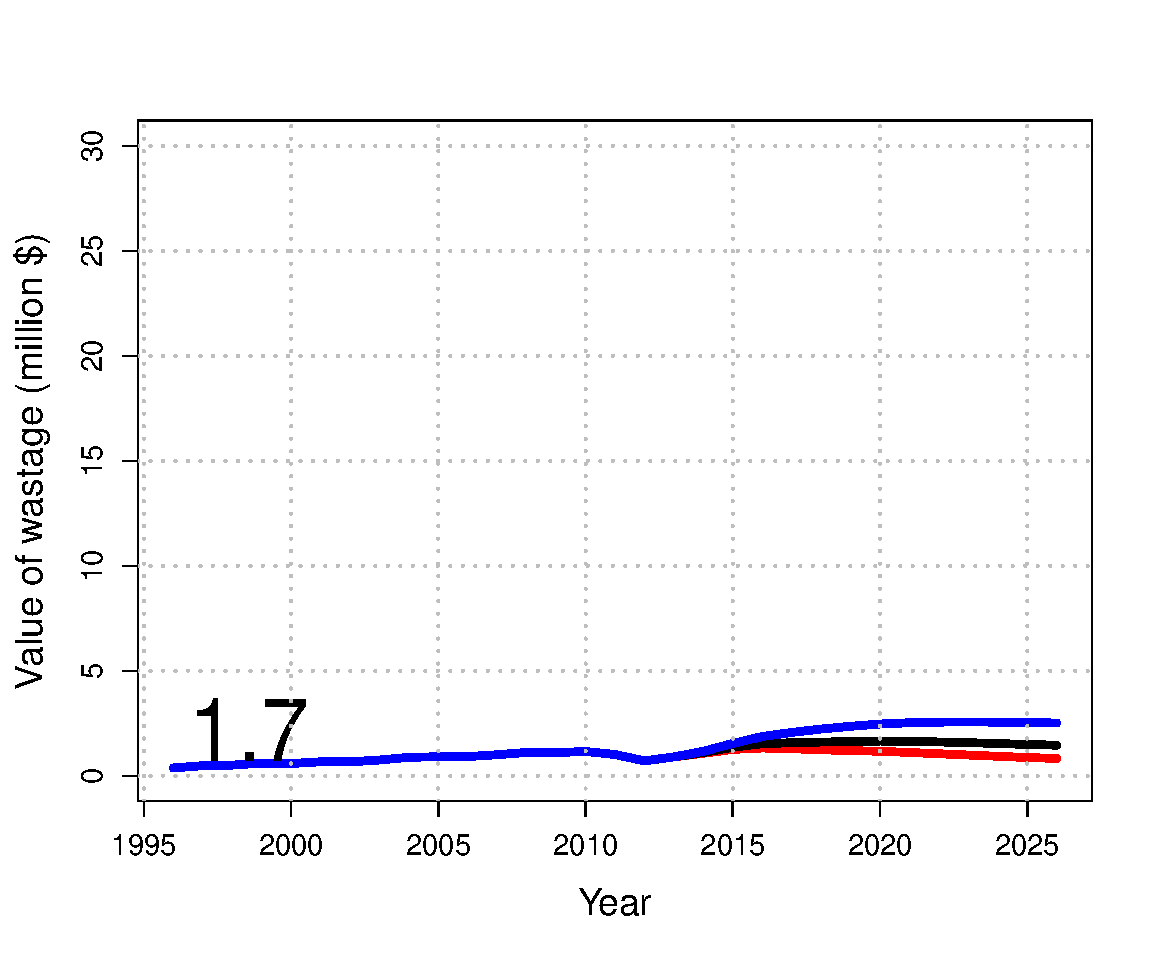
\includegraphics[height=1.5in]{../FIGURES/SIZELIMIT/fig_26_DI_WVal.pdf}
		                                                              
		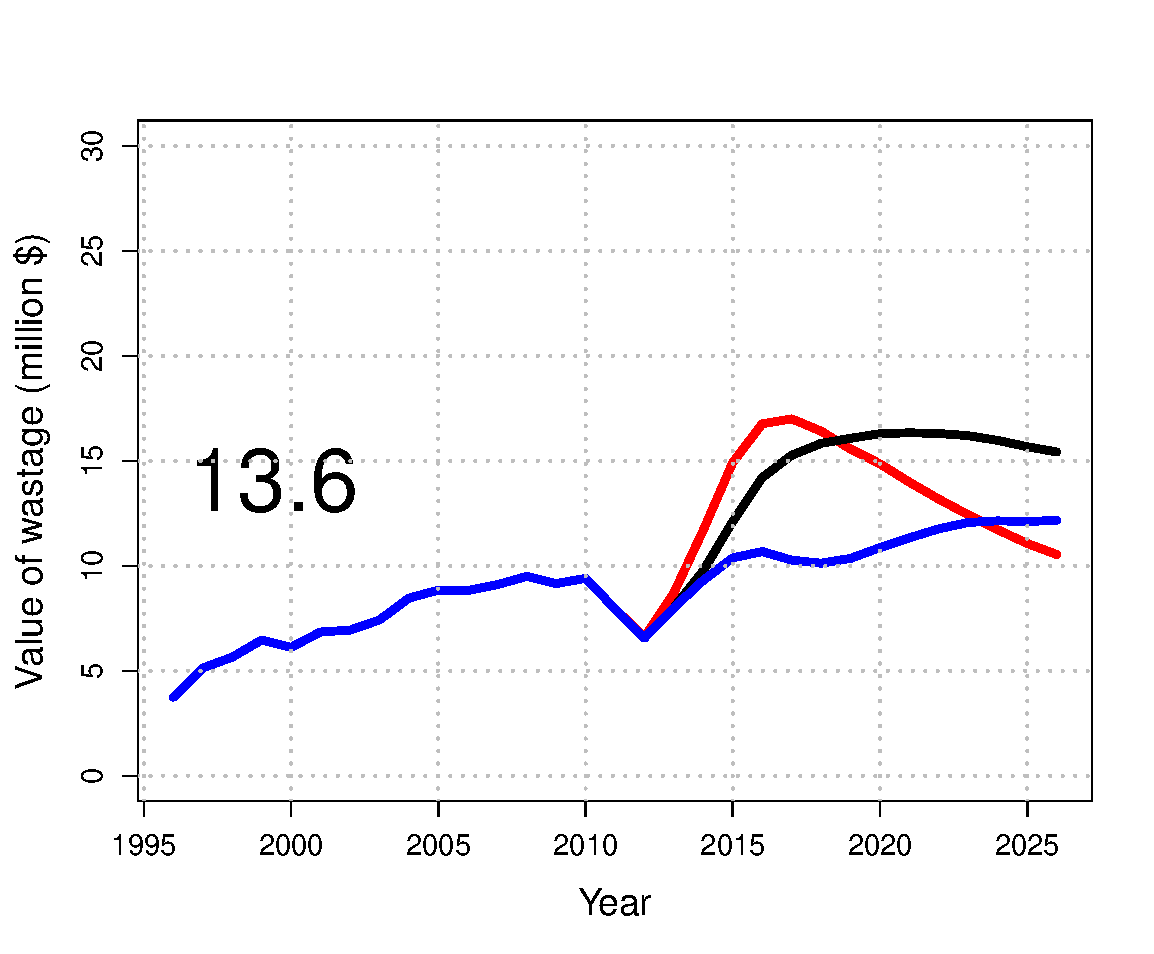
\includegraphics[height=1.5in]{../FIGURES/SIZELIMIT/fig_32_DD_WVal.pdf}
		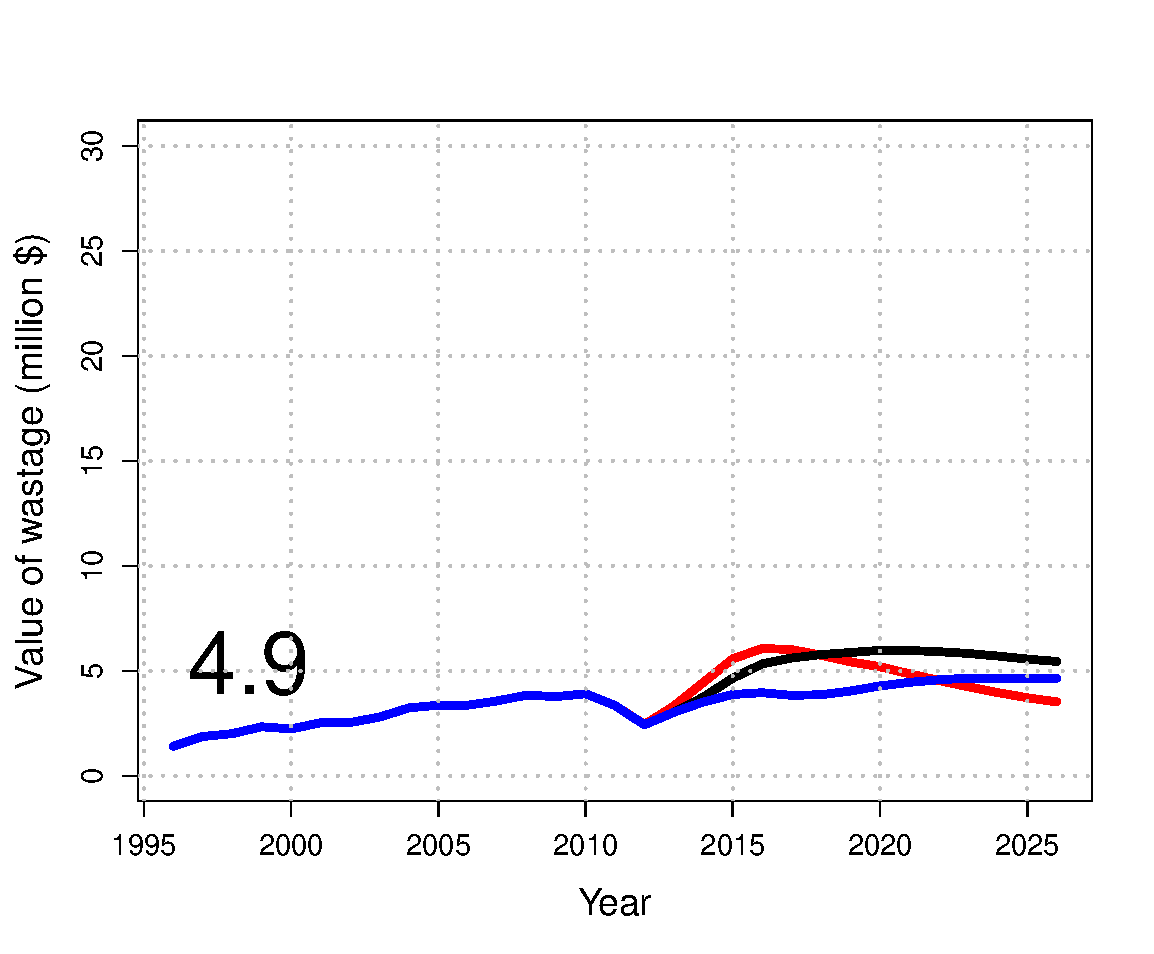
\includegraphics[height=1.5in]{../FIGURES/SIZELIMIT/fig_29_DD_WVal.pdf}
		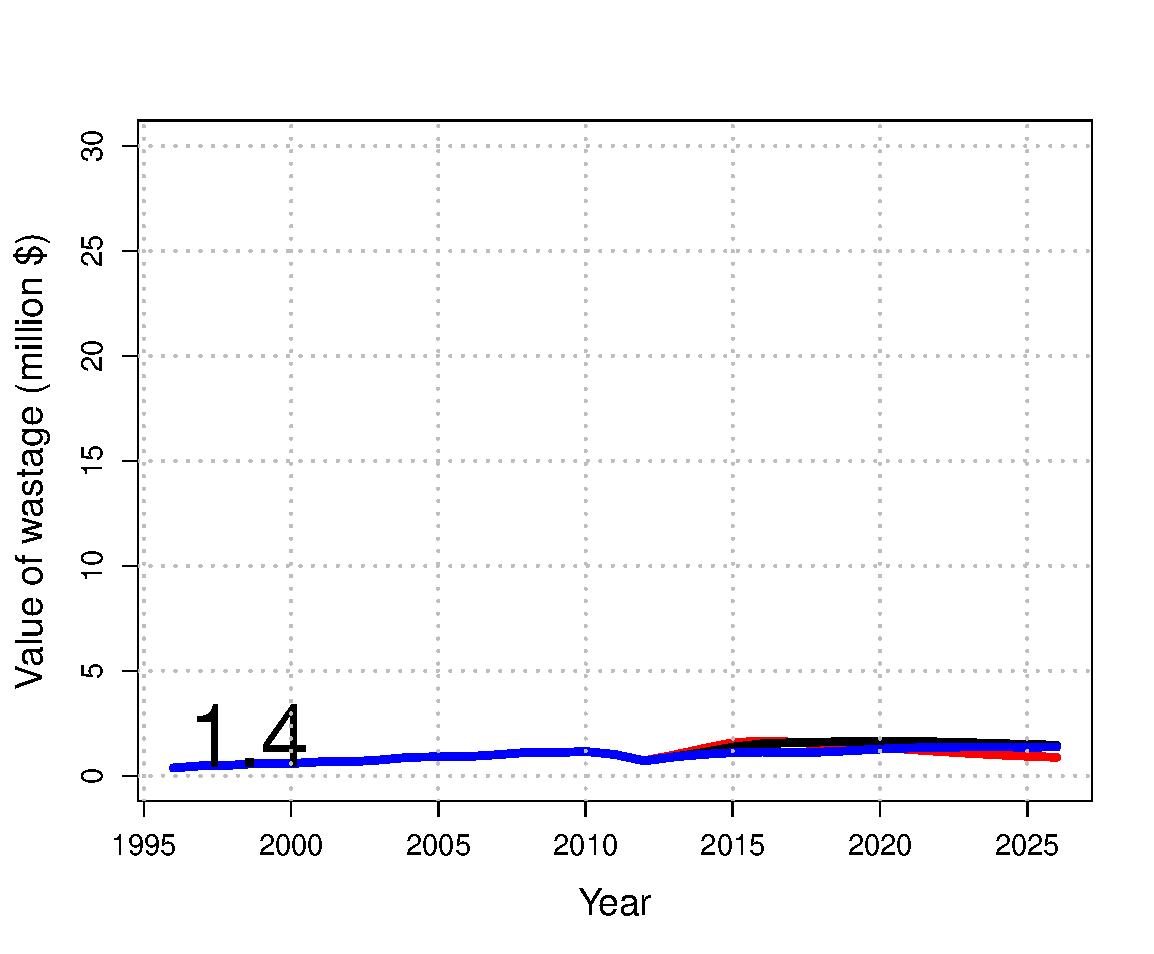
\includegraphics[height=1.5in]{../FIGURES/SIZELIMIT/fig_26_DD_WVal.pdf}
	\caption{Value of commercial wastage under the assumptions of density-independent growth (top row) and density-dependent growth (bottom row) for 32 inch (left), 29 inch (middle), and 26 inch (right) size limits.  Poor, average, and good recruitment are denoted by red, black and blue lines, respectively.  Value on each panel corresponds to 2020-2025 average over 3 recruitment hypotheses.}
	\label{fig:FIGURES_SIZELIMIT_fig_32_DI_WVal}
\end{figure}

Not all of the commercial fish that are captured die due to handling mortality; the estimated discard mortality rate for this fishery is 16\%.  The average simulated coastwide value of the commercial fish landed that are of sublegal size (assuming \$5.00 per pound) under a 32 inch size limit is \$91 million.  Reducing the size limit to 29 and 26 inches reduces the value of sublegal fish captured to \$33 and \$9 million, respectively (Figure \ref{fig:FIGURES_SIZELIMIT_fig_32_DI_DVal}).  



\begin{figure}[htbp]
	\centering
		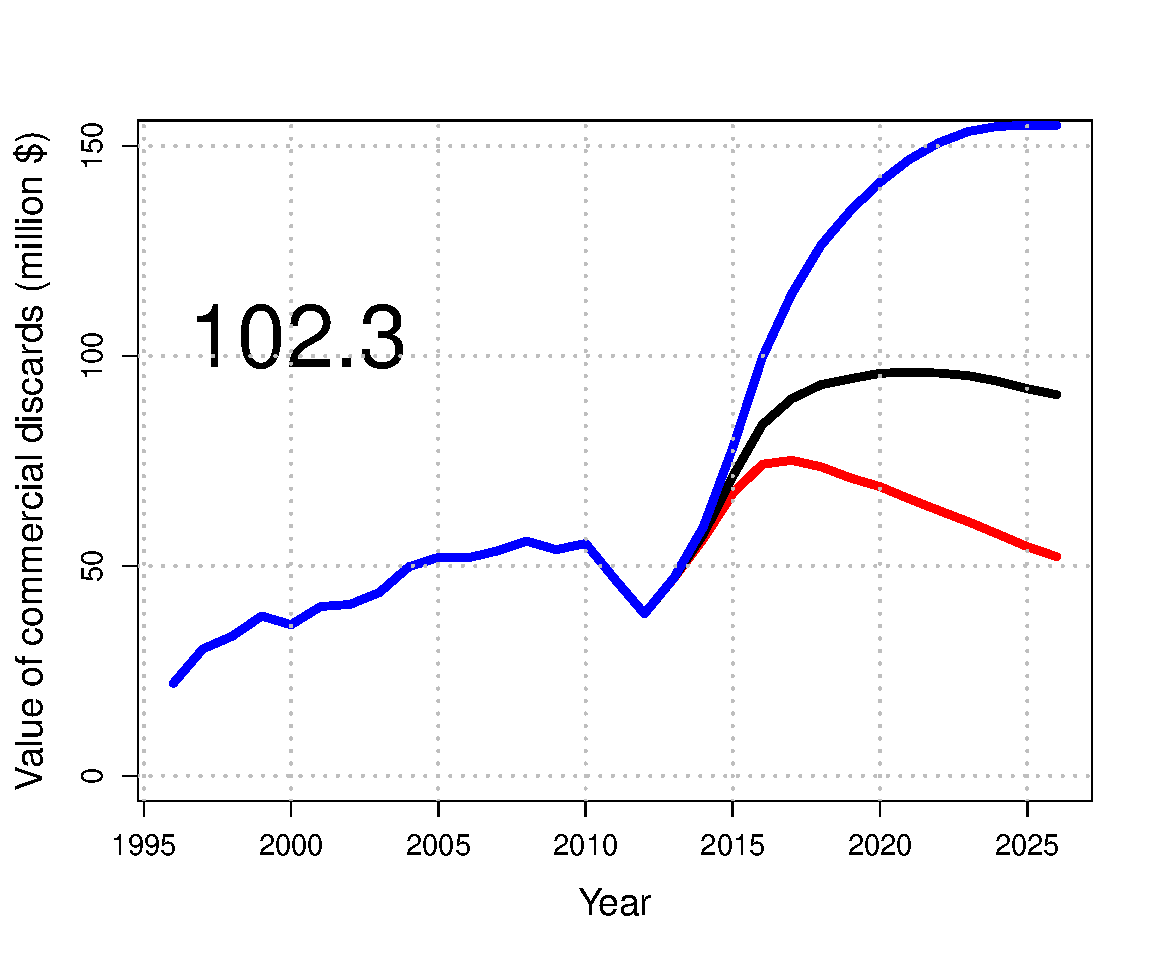
\includegraphics[height=1.5in]{../FIGURES/SIZELIMIT/fig_32_DI_DVal.pdf}
		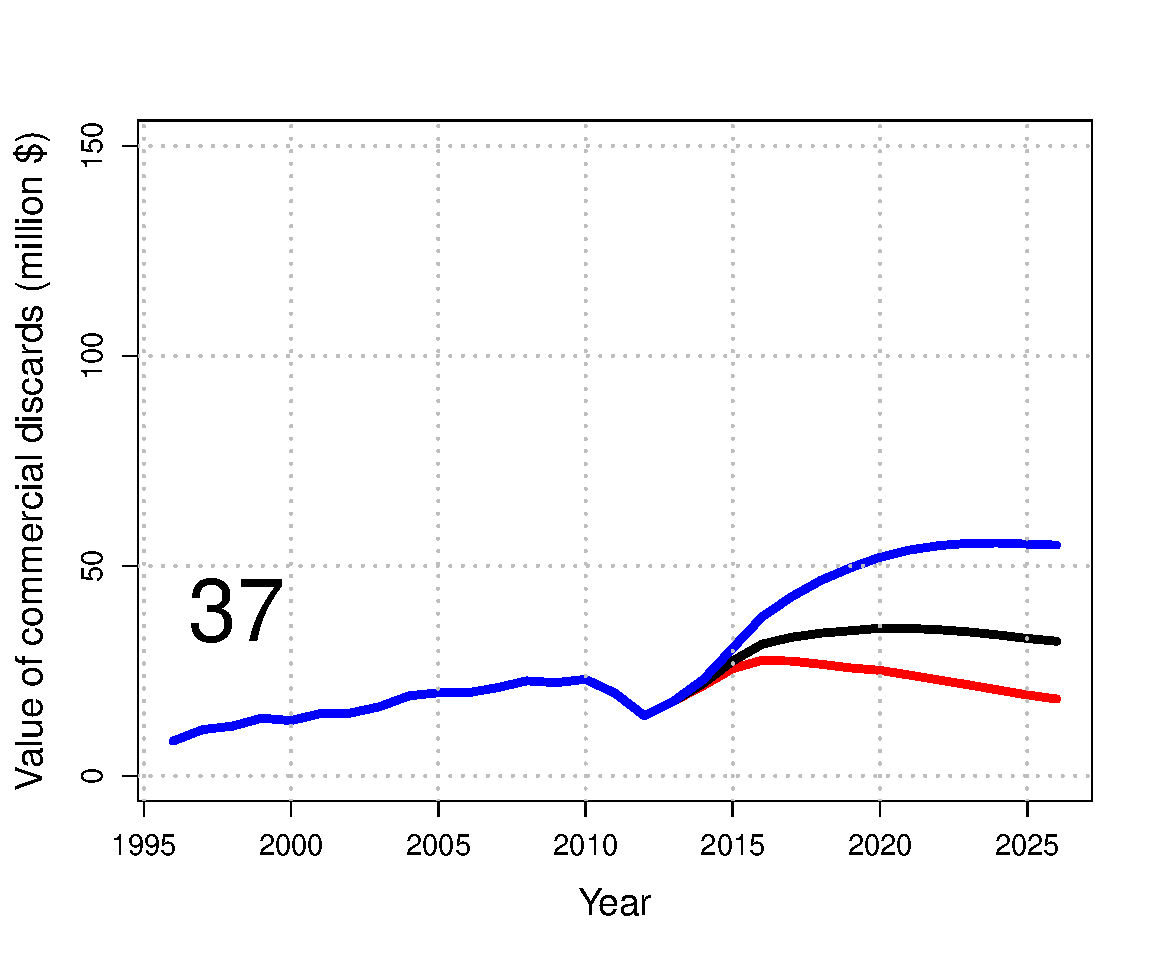
\includegraphics[height=1.5in]{../FIGURES/SIZELIMIT/fig_29_DI_DVal.pdf}
		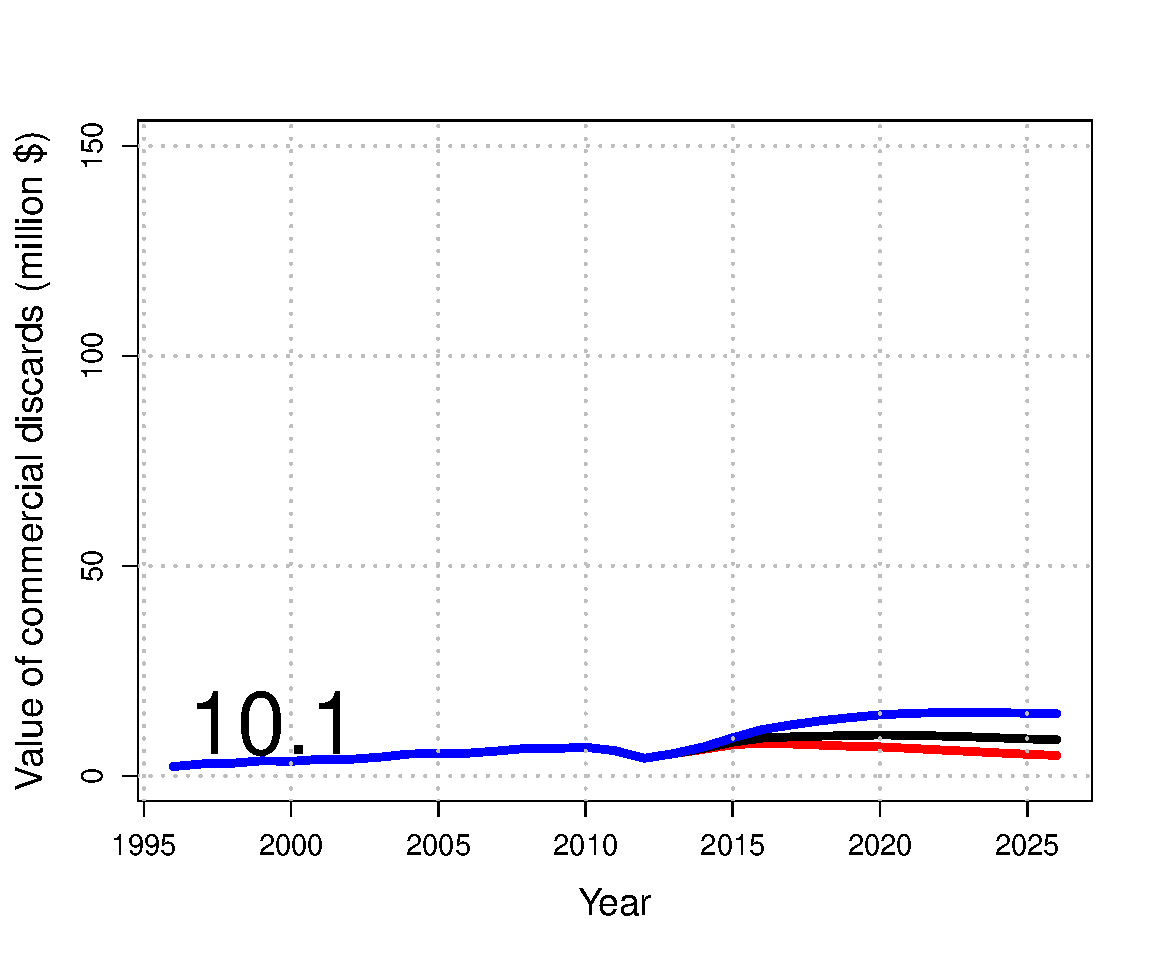
\includegraphics[height=1.5in]{../FIGURES/SIZELIMIT/fig_26_DI_DVal.pdf}
		                                                              
		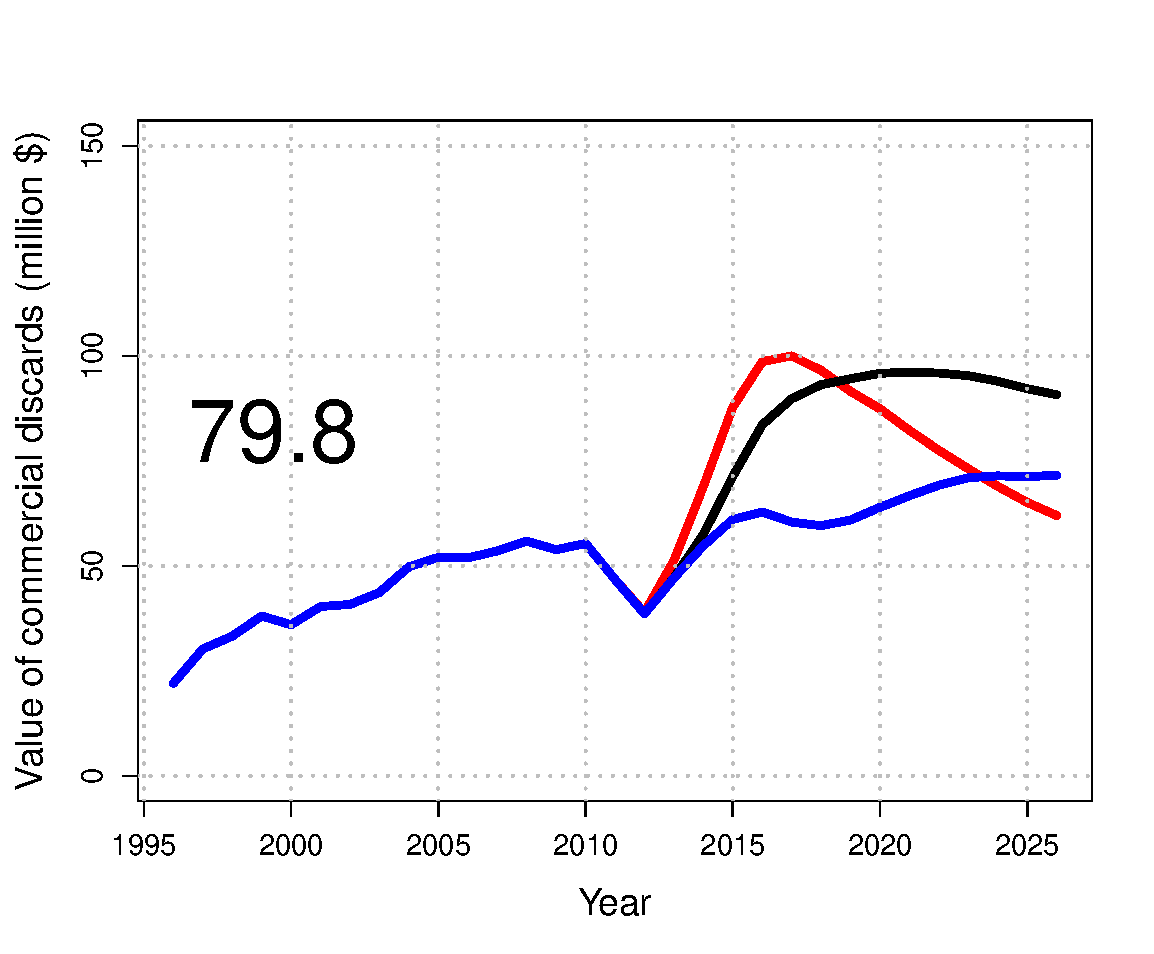
\includegraphics[height=1.5in]{../FIGURES/SIZELIMIT/fig_32_DD_DVal.pdf}
		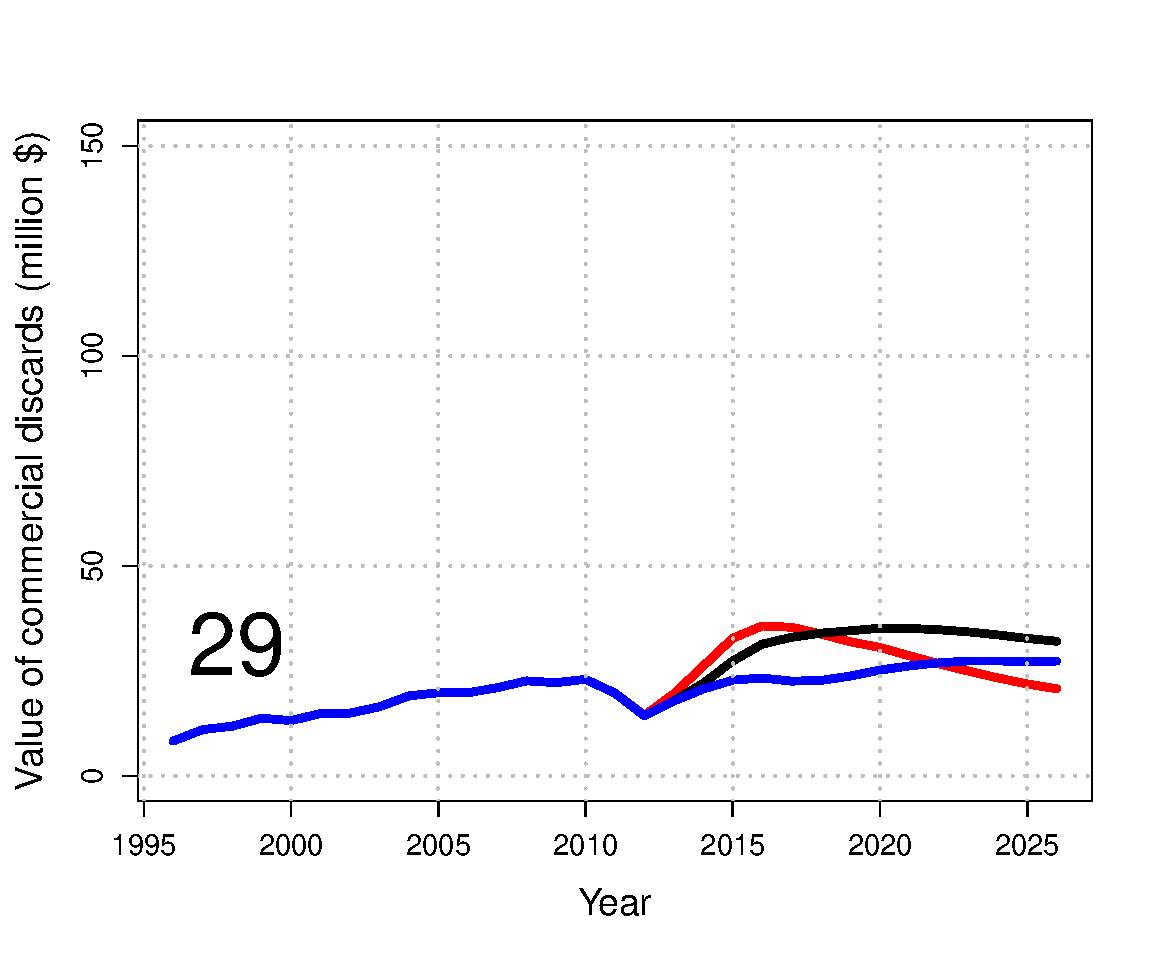
\includegraphics[height=1.5in]{../FIGURES/SIZELIMIT/fig_29_DD_DVal.pdf}
		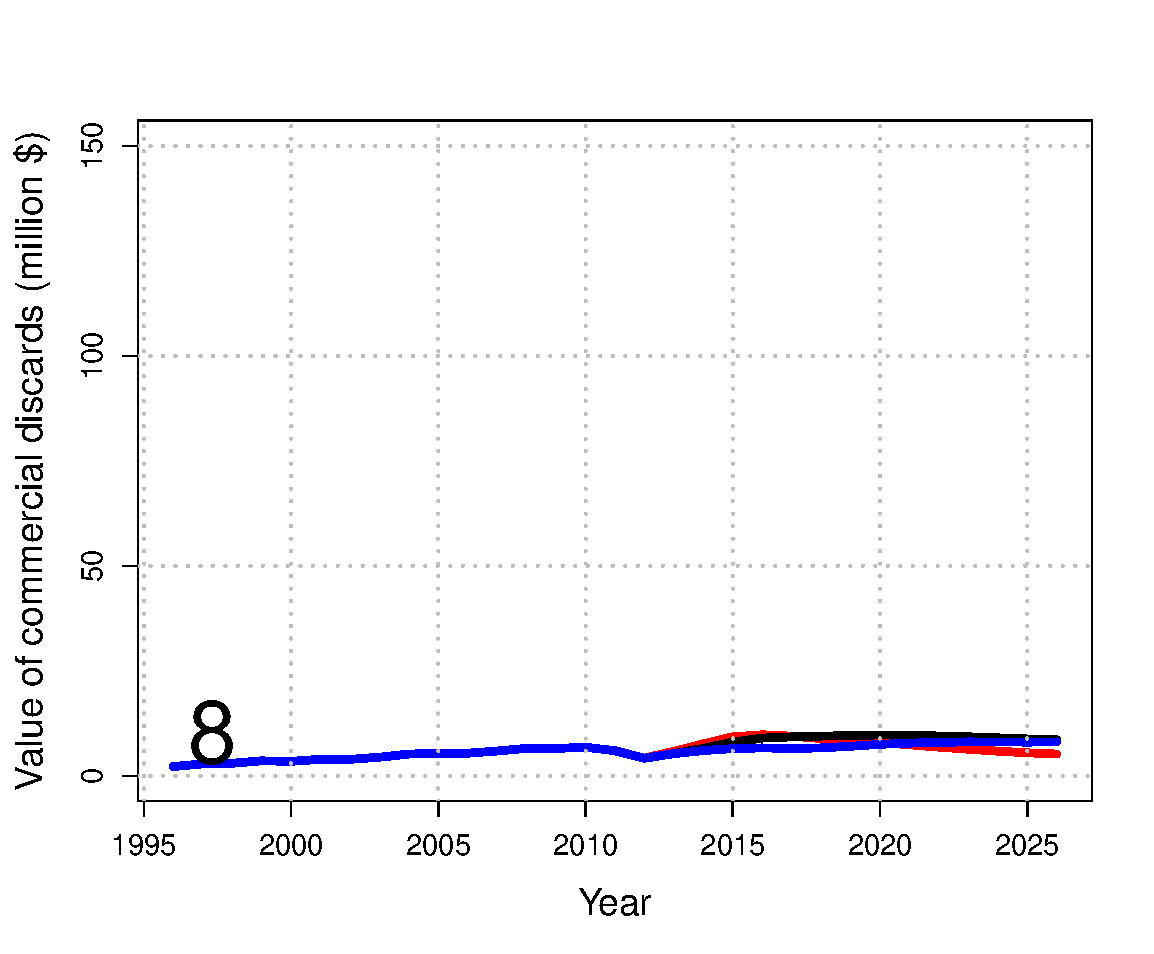
\includegraphics[height=1.5in]{../FIGURES/SIZELIMIT/fig_26_DD_DVal.pdf}
	\caption{Value of all commercial sublegal size fish under the assumptions of density-independent growth (top row) and density-dependent growth (bottom row) for 32 inch (left), 29 inch (middle), and 26 inch (right) size limits.  Poor, average, and good recruitment are denoted by red, black and blue lines, respectively.  Value on each panel corresponds to 2020-2025 average over 3 recruitment hypotheses.}
	\label{fig:FIGURES_SIZELIMIT_fig_32_DI_DVal}
\end{figure}

The practice of discarding sublegal size fish can be considered an added cost associated with handling time and lower capture probabilities of legal size fish due to competition for hooks.  These cost can be significant and would increase or decrease with changes in size limits as shown in Figure \ref{fig:FIGURES_SIZELIMIT_fig_32_DI_DVal}.  A proximate measure for fishing efficiency from an economic standpoint of view is can be defined as:
\[1-\frac{\mbox{value of discards}}{\mbox{value of landings}}.\]
This term is a measure of the economic efficiency and under a 32 inch size limit this value is roughly 87\% in comparison to 98.7\% under a 26 inch size limit (Table \ref{table:SizeLimit_SummaryTable}).  Another proximate measure is the handling efficiency, or simply what fraction of the fish captured that are retained.  Under  a 32 inch size-limit the average simulated handling efficiency between 2020-2025 is 40\%.  In other words, 60 out of 100 captured halibut are below the minimum legal size and are discarded.  Whereas, under a 26 inch size limit the handling efficiency increases to 91\%, or 9 out of 100 captured halibut are below the minimum legal size (Table \ref{table:SizeLimit_SummaryTable}).


\begin{table}
	\caption{Summary of simulated performance measures for three alternative size limit policies averaged over 3 recruitment levels and 2 alternative hypthoses about halibut growth.}
	\label{table:SizeLimit_SummaryTable}
	\begin{center}
		\begin{tabular}{r|c|c|c}
			\hline
			\multicolumn{1}{l}{{Response (million lb)}} & {32'' MSL} & {29'' MSL}  & {26'' MSL } \\
			\hline
			EBio       & 633     & 634      & 635    \\
			Yield      & 101     & 101.25   & 101.4  \\
			Wastage      & {2.494}   & {0.925}    & {0.260}  \\
			\hline
			\multicolumn{4}{l}{{Response (million)}}\\
			\hline
			Landed Value     & \$684.7 & \$683.6  & \$683  \\
			{Waste Value\footnote{Money you cannot recover in the future} }
			 & {\$15.5}&{\$5.6} &{\$1.55} \\
			Discard Value\footnote{Extra cost incurred to throw away these fish.}
			& \$91 & \$33 & \$9\\
			\hline 
			Efficiency & 86.7\%  & 95.2\% & 98.7\% \\
			Handling Efficiency & 40\% & 66\%  & 91\%\\
			\hline
		\end{tabular}
	\end{center}
\end{table}

% subsection impacts_of_msl_on_economic_value (end)

% section results (end)














